\section{Appendix}

\begin{table}[H]
  \centering
  \caption{\label{tab:obs_per_quarter}Number of observations per quarter}
  \centering
  \begin{threeparttable}
    \begin{tabular}[t]{lccc}
      \toprule
      Trimester & Weighted observations & Unweighted observations & Occupations \\
      \midrule
      2020 Q3   & 46,569,449            & 110,385                 & 422         \\
      2020 Q4   & 48,647,210            & 139,327                 & 422         \\
      2021 Q1   & 48,770,663            & 136,762                 & 422         \\
      2021 Q2   & 50,462,809            & 153,040                 & 422         \\
      2021 Q3   & 50,253,742            & 168,719                 & 422         \\
      2021 Q4   & 51,100,235            & 173,620                 & 422         \\
      2022 Q1   & 50,763,871            & 160,125                 & 422         \\
      2022 Q2   & 51,742,781            & 163,873                 & 422         \\
      2022 Q3   & 51,702,338            & 161,068                 & 422         \\
      2022 Q4   & 52,595,404            & 162,520                 & 422         \\
      2023 Q1   & 52,744,085            & 184,138                 & 422         \\
      2023 Q2   & 52,590,073            & 176,258                 & 422         \\
      2023 Q3   & 53,007,959            & 176,189                 & 422         \\
      2023 Q4   & 53,495,100            & 173,657                 & 422         \\
      2024 Q1   & 53,246,806            & 174,315                 & 422         \\
      2024 Q2   & 53,366,181            & 176,022                 & 422         \\
      2024 Q3   & 53,390,082            & 174,369                 & 422         \\
      2024 Q4   & 53,504,313            & 173,182                 & 422         \\
      2025 Q1   & 53,183,827            & 171,360                 & 422         \\
      2025 Q2   & 53,425,948            & 172,173                 & 422         \\
      2025 Q3   & 53,365,860            & 171,884                 & 422         \\
      2025 Q4   & 53,713,012            & 171,445                 & 422         \\
      2026 Q1   & 53,626,325            & 169,675                 & 422         \\
      2026 Q2   & 53,901,224            & 170,791                 & 422         \\
      \bottomrule
    \end{tabular}
    \begin{tablenotes}
      \item \textit{Note:} Observations are weighted by \glsxtrshort{ENOE} expansion factors. Mean (std. dev.) across quarters: weighted observations = 52,048,721 (1,929,482); unweighted observations = 165,204 (16,163)
    \end{tablenotes}
  \end{threeparttable}
\end{table}


\begin{table}[H]
  \centering
  \caption{Classification of Tasks by LLM Exposure \citep{eloundou2023gptsgptsearlylook}}
  \label{tab:llm_exposure}
  \begin{tabular}{@{}p{0.35\textwidth} p{0.57\textwidth}@{}}
    \toprule
    \textbf{Exposure Category} & \textbf{Definition}                                                                                                                                                                                                                                                                                            \\
    \midrule
    \textbf{E0 (No Exposure)}
                               & LLM use does not reduce the time required to complete the activity or task by at least 50\% while maintaining equivalent quality, or it reduces the quality of the output.                                                                                                                                     \\[0.4em]

    \textbf{E1 (Direct Exposure)}
                               & The described LLM, accessed directly through ChatGPT or the OpenAI Playground, can reduce the time required to complete the activity or task by at least 50\% while maintaining equivalent quality.                                                                                                            \\[0.4em]

    \textbf{E2 (LLM+ Exposure)}
                               & Access to the LLM alone cannot reduce task completion time by at least 50\% while maintaining equivalent quality. However, additional software developed on top of the LLM could achieve this reduction. This category also includes tasks that can be accelerated through access to image-generation systems. \\
    \bottomrule
  \end{tabular}

  \vspace{0.3em}
  \begin{minipage}{0.95\textwidth}
    \footnotesize
    \textit{Note:} Equivalent quality means that a third party, typically the recipient of the output, would not notice or care that the task was completed with LLM assistance. In the original classification, access to image-generation capabilities is categorized separately as E3 to facilitate annotation; E2 and E3 are combined for the main analyses.
  \end{minipage}
\end{table}

\begin{figure}[H]
  \centering
  \caption{Distribution of exposure measures across occupations}
  \begin{subfigure}[b]{0.7\textwidth}
    \centering
    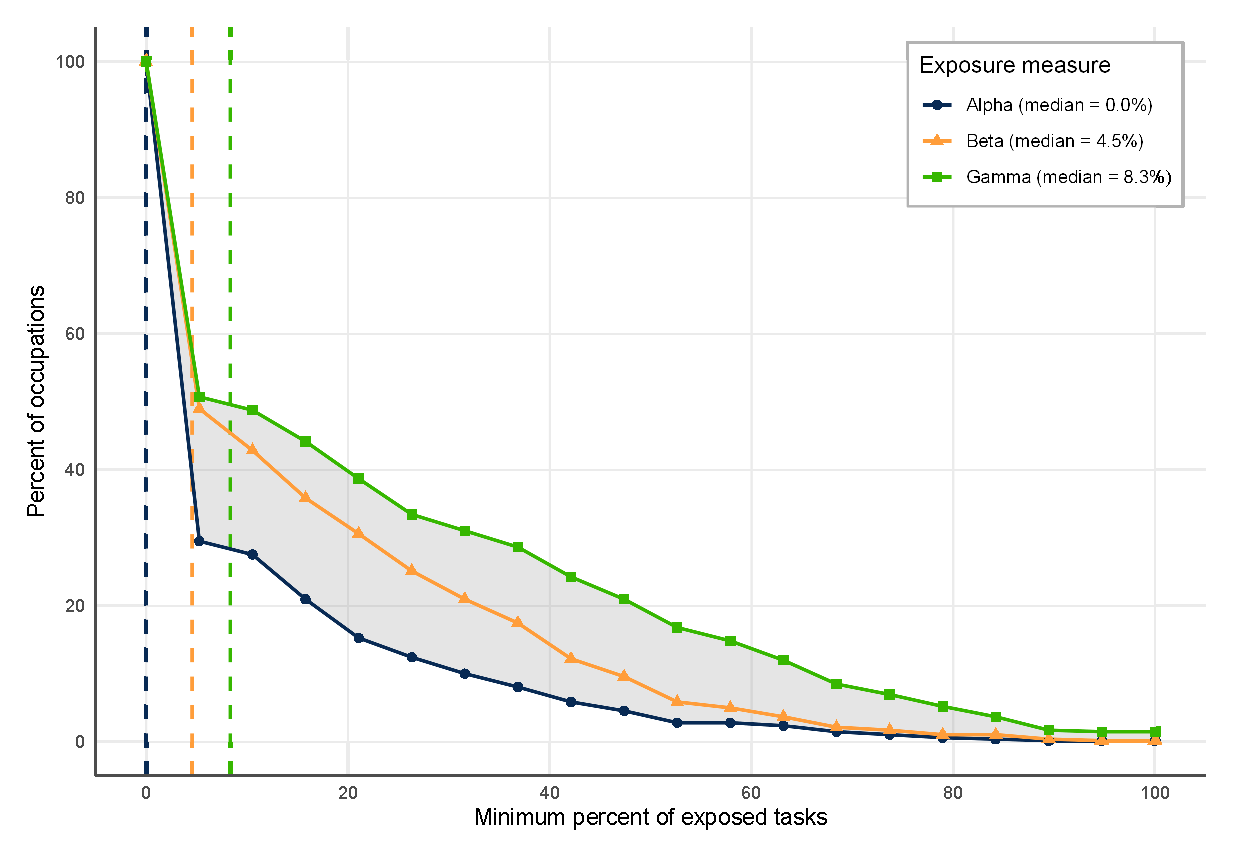
\includegraphics[width=\textwidth]{Figures/exposure_dist_gpt.eps}
    \caption{GPT-4o}
    \label{fig:exposure_dist_gpt}
  \end{subfigure}
  \medskip
  \begin{subfigure}[b]{0.7\textwidth}
    \centering
    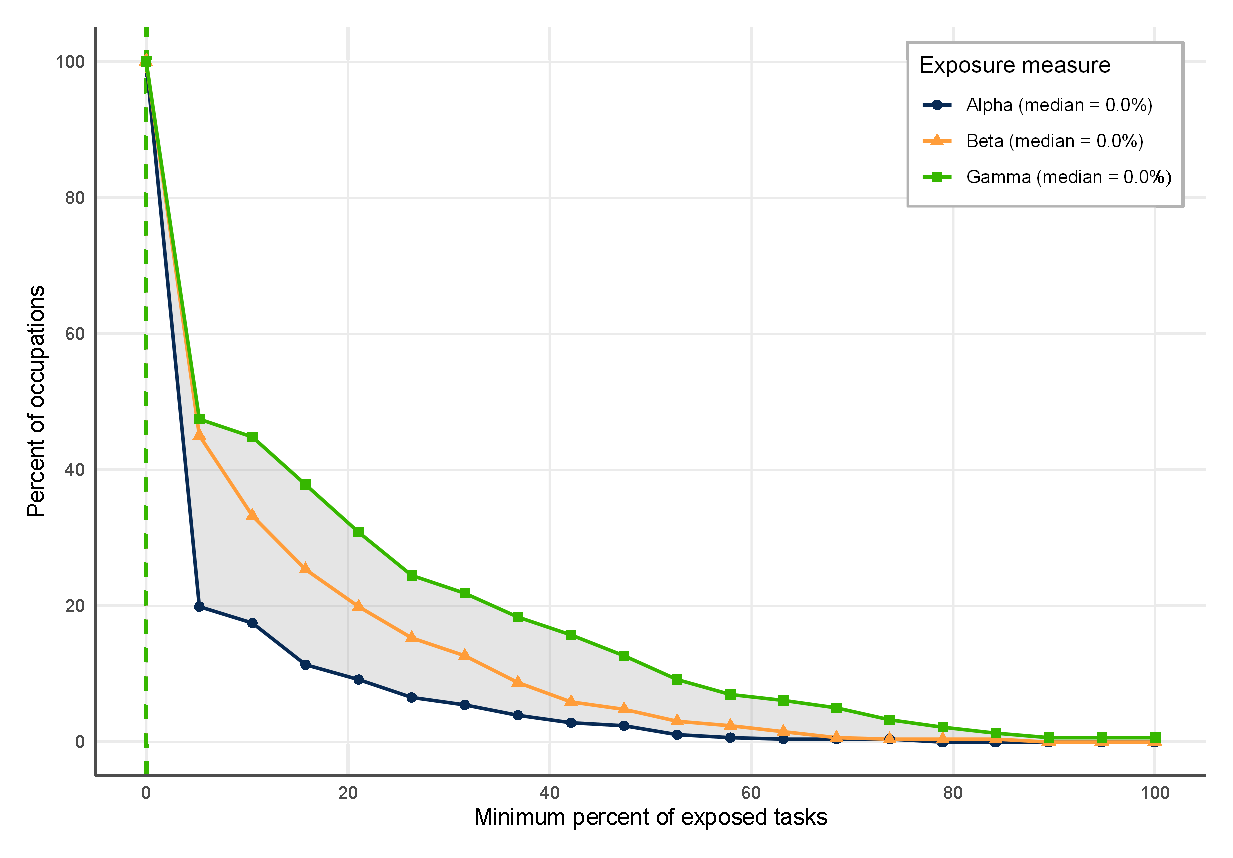
\includegraphics[width=\textwidth]{Figures/exposure_dist_human.eps}
    \caption{Human}
    \label{fig:exposure_dist_human}
  \end{subfigure}
  \medskip
  \label{fig:exposure_dist}
  \begin{minipage}{\textwidth}
    \small
    \textit{Note:} The plotted dashed lines indicate the median associated with each measure.
  \end{minipage}
\end{figure}


\begin{figure}[H]
  \centering
  \caption{Treatment group by exposure measure}
  \begin{subfigure}[b]{0.7\textwidth}
    \centering
    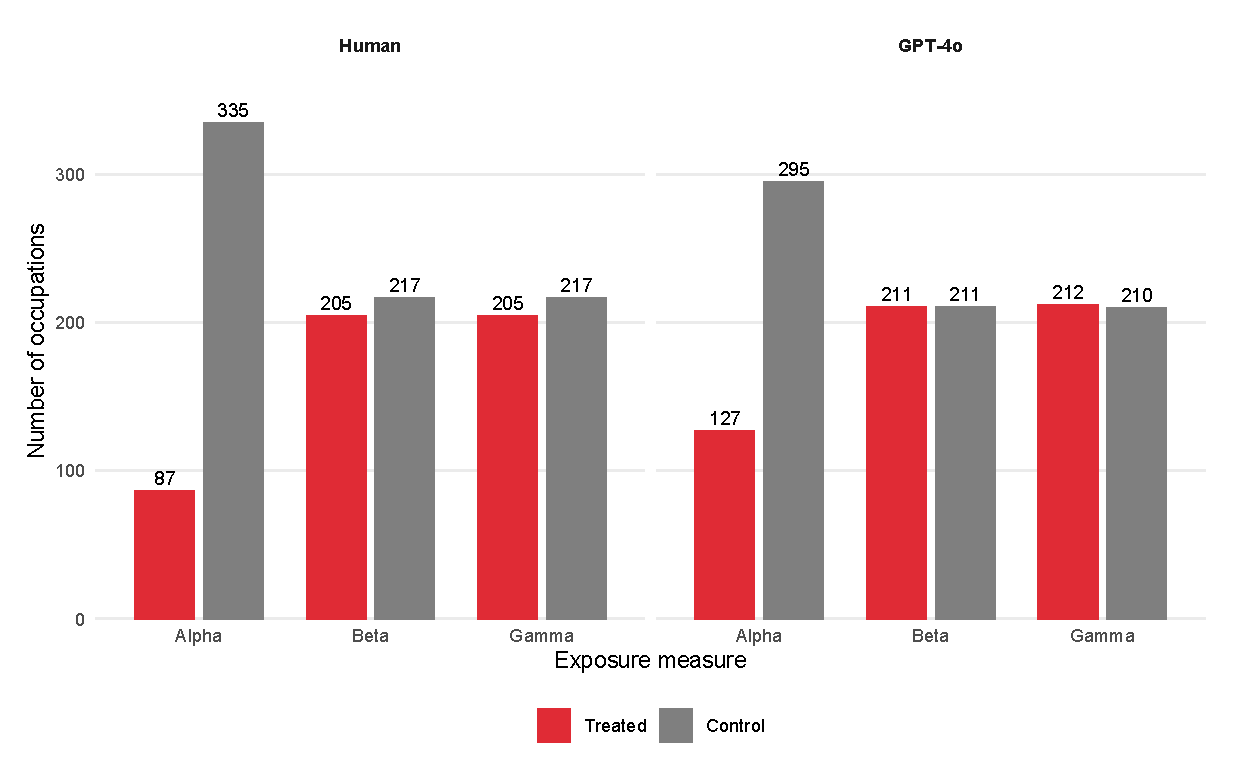
\includegraphics[width=\textwidth]{Figures/occupations_by_treatment.eps}
    \caption{Occupation}
    \label{fig:occupation_by_treat}
  \end{subfigure}
  \medskip
  \begin{subfigure}[b]{0.7\textwidth}
    \centering
    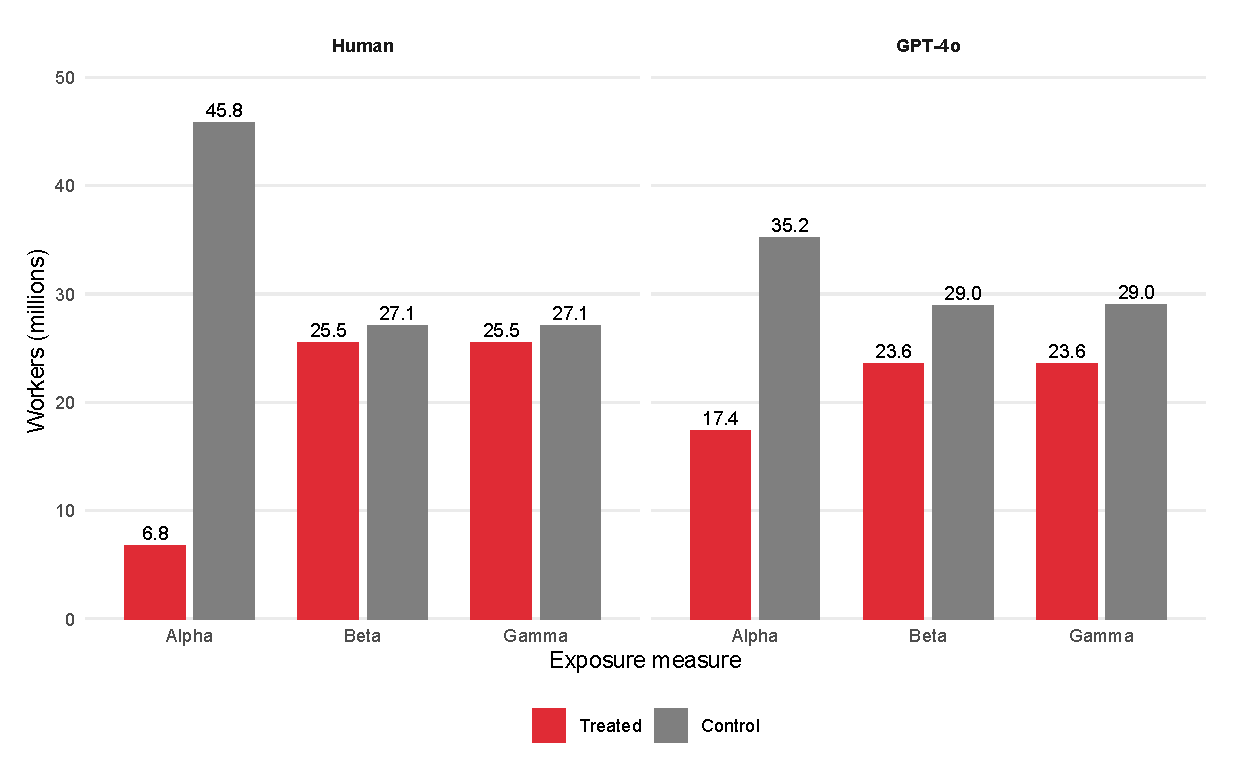
\includegraphics[width=\textwidth]{Figures/workers_by_treatment.eps}
    \caption{Workers}
    \label{fig:workers_by_treat}
  \end{subfigure}
  \medskip
  \label{fig:occupations_and_workers_by_treat}
  \begin{minipage}{\textwidth}
    \small
    \textit{Note:} Treated occupations are the ones above the median exposure. Number of workers are computed using the standard \glsxtrshort{ENOE} weights for the treatment quarter (2022 Q4).
  \end{minipage}
\end{figure}


\begin{figure}[H]
  \centering
  \caption{Overlap between treatment groups matrix}
  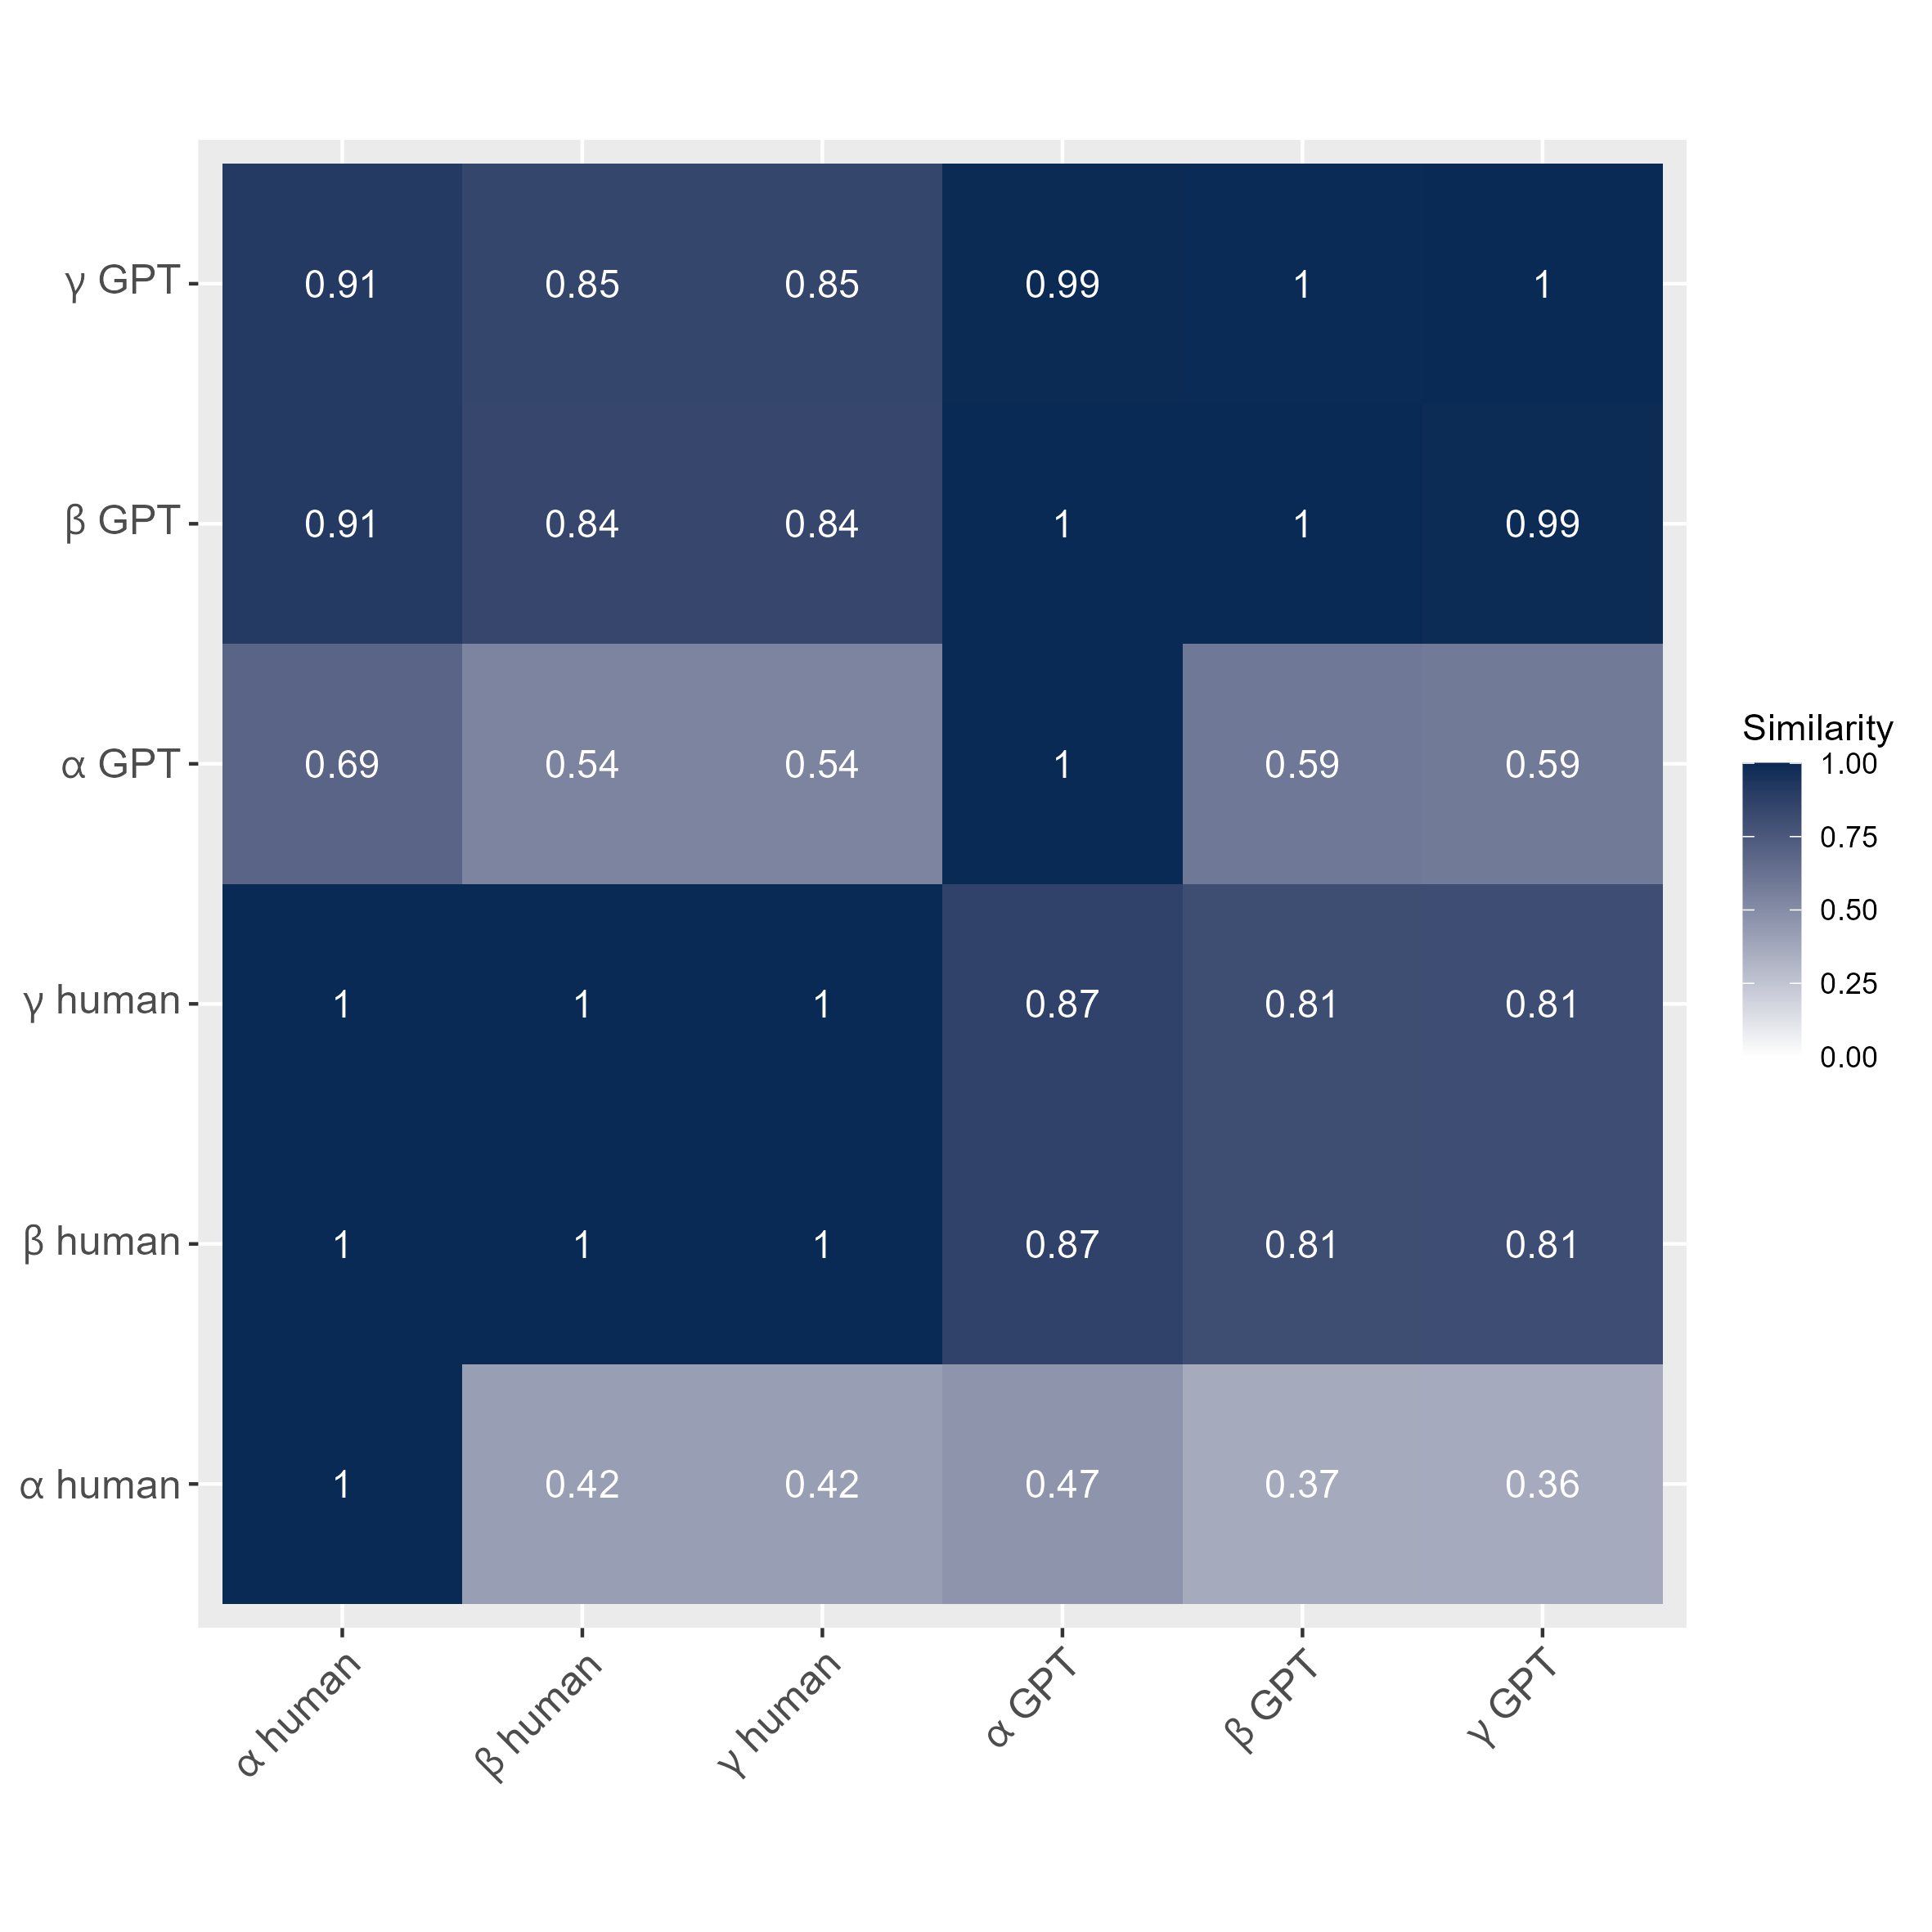
\includegraphics[width=0.7\linewidth]{Figures/matrix.png}
  \label{fig:matrix_overlap}
  \begin{minipage}{\textwidth}
    \small
    \textit{Note:} Share of occupations treated under the x axis measure that are also treated under the y axis measure.
  \end{minipage}
\end{figure}

\begin{table}[H]
  \centering
  \caption{\label{tab:imp_share_gpt}Share of imputed wages (\%) by quarter and treatment group (GPT-4o exposure)}
  \centering
  \resizebox{\ifdim\width>\linewidth\linewidth\else\width\fi}{!}{
    \begin{threeparttable}
      \begin{tabular}[t]{lcccc}
        \toprule
        \multicolumn{1}{c}{ } & \multicolumn{2}{c}{Alpha} & \multicolumn{2}{c}{Beta}                     \\
        \cmidrule(l{3pt}r{3pt}){2-3} \cmidrule(l{3pt}r{3pt}){4-5}
        Quarter               & Treated                   & Control                  & Treated & Control \\
        \midrule
        2020 Q3               & 37.5                      & 24.6                     & 36.7    & 22.4    \\
        2020 Q4               & 36.4                      & 23.6                     & 35.7    & 21.2    \\
        2021 Q1               & 34.7                      & 23.0                     & 34.2    & 20.7    \\
        2021 Q2               & 37.5                      & 25.0                     & 37.1    & 22.4    \\
        2021 Q3               & 37.8                      & 25.1                     & 37.5    & 22.5    \\
        \addlinespace
        2021 Q4               & 38.3                      & 25.5                     & 38.1    & 22.7    \\
        2022 Q1               & 36.0                      & 23.8                     & 35.5    & 21.4    \\
        2022 Q2               & 38.6                      & 25.3                     & 37.6    & 23.1    \\
        2022 Q3               & 39.4                      & 25.9                     & 38.7    & 23.4    \\
        2022 Q4               & 39.9                      & 25.8                     & 39.0    & 23.3    \\
        \addlinespace
        2023 Q1               & 39.0                      & 26.1                     & 38.5    & 23.6    \\
        2023 Q2               & 40.3                      & 26.4                     & 39.6    & 23.8    \\
        2023 Q3               & 39.8                      & 27.0                     & 39.4    & 24.4    \\
        2023 Q4               & 40.3                      & 27.4                     & 40.1    & 24.7    \\
        2024 Q1               & 38.7                      & 26.7                     & 38.3    & 24.2    \\
        \addlinespace
        2024 Q2               & 40.6                      & 27.8                     & 40.1    & 25.1    \\
        2024 Q3               & 40.9                      & 27.8                     & 40.3    & 25.4    \\
        2024 Q4               & 44.5                      & 30.6                     & 43.8    & 28.0    \\
        2025 Q1               & 47.3                      & 33.3                     & 47.0    & 30.4    \\
        2025 Q2               & 48.9                      & 35.3                     & 48.3    & 32.6    \\
        \addlinespace
        2025 Q3               & 48.9                      & 35.7                     & 48.6    & 32.9    \\
        2025 Q4               & 44.4                      & 31.8                     & 44.0    & 29.3    \\
        2026 Q1               & 37.2                      & 25.4                     & 36.8    & 23.0    \\
        2026 Q2               & 39.9                      & 27.3                     & 39.3    & 25.1    \\
        \bottomrule
      \end{tabular}
      \begin{tablenotes}
        \item \textit{Note: }  Share of workers whose earnings were imputed (PMM), weighted by survey expansion factors.
      \end{tablenotes}
    \end{threeparttable}}
\end{table}

\begin{table}[H]
  \centering
  \caption{\label{tab:imp_share_human} Share of imputed wages (\%) by quarter and treatment group (Human exposure)}
  \centering
  \resizebox{\ifdim\width>\linewidth\linewidth\else\width\fi}{!}{
    \begin{threeparttable}
      \begin{tabular}[t]{lcccc}
        \toprule
        \multicolumn{1}{c}{ } & \multicolumn{2}{c}{Alpha} & \multicolumn{2}{c}{Beta}                     \\
        \cmidrule(l{3pt}r{3pt}){2-3} \cmidrule(l{3pt}r{3pt}){4-5}
        Quarter               & Treated                   & Control                  & Treated & Control \\
        \midrule
        2020 Q3               & 43.1                      & 26.9                     & 35.4    & 23.0    \\
        2020 Q4               & 42.0                      & 25.8                     & 34.7    & 21.7    \\
        2021 Q1               & 40.0                      & 24.9                     & 33.2    & 21.1    \\
        2021 Q2               & 42.4                      & 27.2                     & 36.0    & 22.8    \\
        2021 Q3               & 43.3                      & 27.3                     & 36.1    & 23.1    \\
        \addlinespace
        2021 Q4               & 44.1                      & 27.5                     & 36.5    & 23.5    \\
        2022 Q1               & 41.9                      & 25.7                     & 33.9    & 22.3    \\
        2022 Q2               & 43.8                      & 27.6                     & 35.9    & 24.0    \\
        2022 Q3               & 45.9                      & 28.1                     & 37.1    & 24.0    \\
        2022 Q4               & 45.7                      & 28.1                     & 37.3    & 24.1    \\
        \addlinespace
        2023 Q1               & 44.7                      & 28.2                     & 36.8    & 24.4    \\
        2023 Q2               & 45.3                      & 28.9                     & 38.1    & 24.4    \\
        2023 Q3               & 45.3                      & 29.1                     & 38.2    & 24.7    \\
        2023 Q4               & 45.6                      & 29.6                     & 38.9    & 25.1    \\
        2024 Q1               & 43.9                      & 28.7                     & 36.7    & 25.0    \\
        \addlinespace
        2024 Q2               & 46.1                      & 29.9                     & 38.5    & 25.9    \\
        2024 Q3               & 47.2                      & 30.0                     & 38.9    & 25.9    \\
        2024 Q4               & 50.0                      & 33.1                     & 42.0    & 29.1    \\
        2025 Q1               & 52.2                      & 36.0                     & 44.9    & 31.8    \\
        2025 Q2               & 54.6                      & 37.7                     & 46.8    & 33.5    \\
        \addlinespace
        2025 Q3               & 54.1                      & 38.1                     & 47.1    & 33.7    \\
        2025 Q4               & 49.3                      & 34.1                     & 42.8    & 29.8    \\
        2026 Q1               & 42.9                      & 27.4                     & 35.6    & 23.6    \\
        2026 Q2               & 45.3                      & 29.6                     & 38.0    & 25.7    \\
        \bottomrule
      \end{tabular}
      \begin{tablenotes}
        \item \textit{Note: }Share of workers whose earnings were imputed (PMM), weighted by survey expansion factors.
      \end{tablenotes}
    \end{threeparttable}}
\end{table}

\begin{figure}[H]
  \centering
  \caption{Difference in imputed wage share}
  \begin{subfigure}[b]{0.7\textwidth}
    \centering
    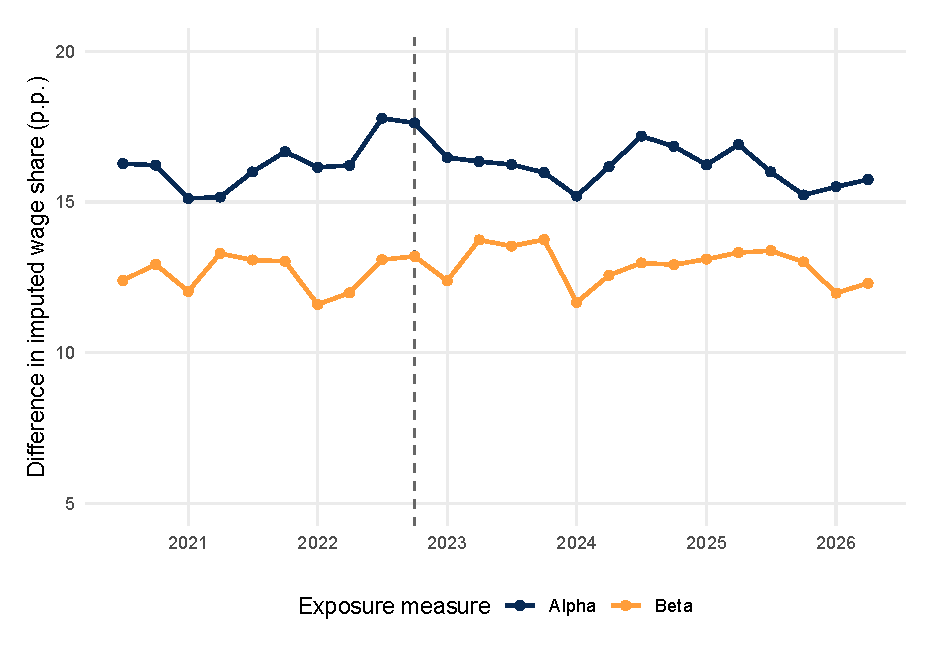
\includegraphics[width=\textwidth]{Figures/imp_share_gap_human.eps}
    \caption{Human}
    \label{fig:imp_share_gap_human}
  \end{subfigure}
  \medskip
  \begin{subfigure}[b]{0.7\textwidth}
    \centering
    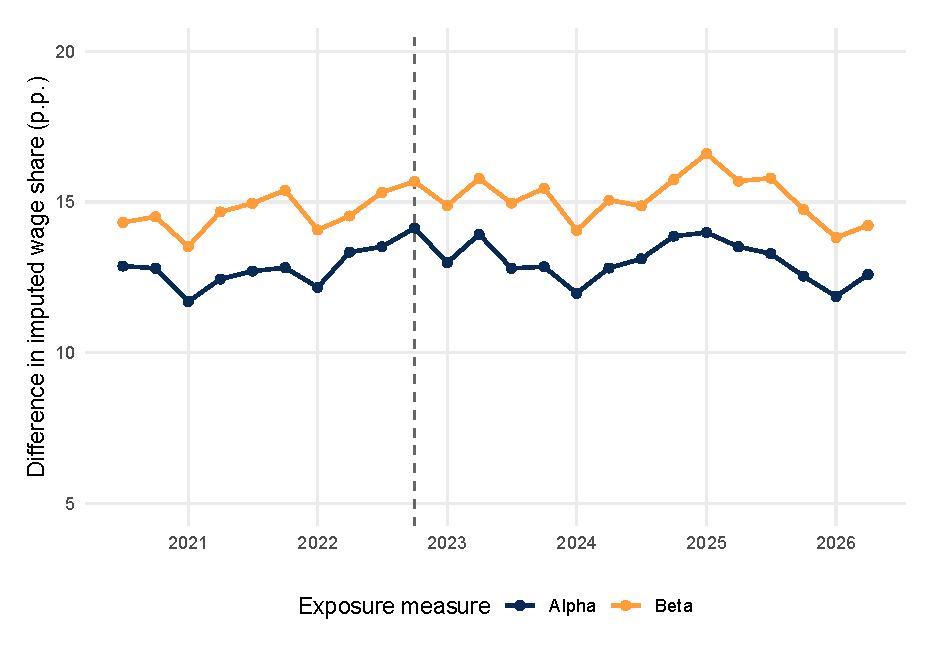
\includegraphics[width=\textwidth]{Figures/imp_share_gap_gpt.eps}
    \caption{GPT}
    \label{fig:imp_share_gap_gpt}
  \end{subfigure}
  \medskip
  \label{fig:imp_share_gap}
  \begin{minipage}{\textwidth}
    \small
    \textit{Note:} The figure plots the difference between treated and control occupations in the share of workers whose earnings were imputed (PMM). Panel (a) uses the human exposure measures and panel (b) the GPT-4o measures. Treated occupations are those above the median exposure. Shares are weighted by ENOE expansion factors. The dashed vertical line marks 2022 Q4, the quarter of ChatGPT's release. A flat series indicates that the gap in imputation between treated and control occupations remained constant before and after the treatment period.
  \end{minipage}
\end{figure}


\begin{table}[H]
  \centering
  \caption{\label{tab:sumstats_exposure_alpha_human}Summary statistics by treatment group (Human Alpha)}
  \centering
  \begin{threeparttable}
    \begin{tabular}[t]{lcccc}
      \toprule
      \multicolumn{1}{c}{ }          & \multicolumn{2}{c}{Control} & \multicolumn{2}{c}{Treated}                         \\
      \cmidrule(l{3pt}r{3pt}){2-3} \cmidrule(l{3pt}r{3pt}){4-5}
                                     & Before                      & After                       & Before    & After     \\
      \midrule
      Female (share)                 & 0.387                       & 0.404                       & 0.476     & 0.484     \\
                                     & (0.307)                     & (0.306)                     & (0.213)   & (0.214)   \\
      \addlinespace[3pt]
      Number of workers              & 910,742                     & 955,220                     & 266,830   & 276,887   \\
                                     & (881,588)                   & (949,268)                   & (194,607) & (203,653) \\
      \addlinespace[3pt]
      Number of informal workers     & 641,232                     & 654,980                     & 37,535    & 40,185    \\
                                     & (704,332)                   & (725,615)                   & (26,768)  & (26,522)  \\
      \addlinespace[3pt]
      Social security access (share) & 0.367                       & 0.373                       & 0.731     & 0.727     \\
                                     & (0.339)                     & (0.336)                     & (0.208)   & (0.206)   \\
      \addlinespace[3pt]
      Union member (share)           & 0.382                       & 0.361                       & 0.764     & 0.711     \\
                                     & (0.341)                     & (0.337)                     & (0.288)   & (0.325)   \\
      \addlinespace[3pt]
      Years of schooling             & 10.13                       & 10.42                       & 15.40     & 15.54     \\
                                     & (2.36)                      & (2.31)                      & (1.91)    & (1.97)    \\
      \addlinespace[3pt]
      Age (years)                    & 39.0                        & 39.4                        & 38.6      & 38.8      \\
                                     & (4.1)                       & (4.1)                       & (3.1)     & (3.0)     \\
      \addlinespace[3pt]
      Monthly earnings (MXN)         & 7,179                       & 9,546                       & 11,486    & 14,928    \\
                                     & (3,159)                     & (3,959)                     & (2,769)   & (3,662)   \\
      \addlinespace[3pt]
      Weekly hours worked            & 42.2                        & 41.9                        & 36.7      & 36.9      \\
                                     & (7.2)                       & (7.0)                       & (7.9)     & (7.5)     \\
      \midrule
      Occupations                    & 335                         & 335                         & 87        & 87        \\
      Occupation X quarters          & 3,350                       & 4,690                       & 870       & 1,218     \\
      \bottomrule
    \end{tabular}
    \begin{tablenotes}
      \item \textit{Note: } Occupation by quarter observations. Means weighted by occupation employment, with standard deviations across occupation quarters in parentheses. Treated occupations are the ones above the median exposure. The \textit{Before} column averages 2022 Q4 and earlier and the \textit{After} column 2023 Q1 onward. Monthly earnings are imputed with predictive mean matching (PMM).
    \end{tablenotes}
  \end{threeparttable}
\end{table}


\begin{table}[H]
  \centering
  \caption{\label{tab:sumstats_exposure_beta_human}Summary statistics by treatment group (Human Beta)}
  \centering
  \begin{threeparttable}
    \begin{tabular}[t]{lcccc}
      \toprule
      \multicolumn{1}{c}{ }          & \multicolumn{2}{c}{Control} & \multicolumn{2}{c}{Treated}                             \\
      \cmidrule(l{3pt}r{3pt}){2-3} \cmidrule(l{3pt}r{3pt}){4-5}
                                     & Before                      & After                       & Before      & After       \\
      \midrule
      Female (share)                 & 0.326                       & 0.342                       & 0.476       & 0.491       \\
                                     & (0.323)                     & (0.327)                     & (0.245)     & (0.238)     \\
      \addlinespace[3pt]
      Number of workers              & 727,482                     & 740,650                     & 938,749     & 1,005,057   \\
                                     & (628,573)                   & (614,919)                   & (1,032,570) & (1,140,656) \\
      \addlinespace[3pt]
      Number of informal workers     & 559,929                     & 552,992                     & 570,065     & 601,717     \\
                                     & (631,402)                   & (606,973)                   & (744,545)   & (801,228)   \\
      \addlinespace[3pt]
      Social security access (share) & 0.351                       & 0.355                       & 0.480       & 0.486       \\
                                     & (0.337)                     & (0.335)                     & (0.345)     & (0.338)     \\
      \addlinespace[3pt]
      Union member (share)           & 0.344                       & 0.327                       & 0.540       & 0.504       \\
                                     & (0.335)                     & (0.329)                     & (0.357)     & (0.363)     \\
      \addlinespace[3pt]
      Years of schooling             & 9.49                        & 9.78                        & 12.20       & 12.46       \\
                                     & (2.03)                      & (1.96)                      & (3.04)      & (2.97)      \\
      \addlinespace[3pt]
      Age (years)                    & 39.1                        & 39.7                        & 38.7        & 39.0        \\
                                     & (3.8)                       & (3.8)                       & (4.1)       & (4.2)       \\
      \addlinespace[3pt]
      Monthly earnings (MXN)         & 6,964                       & 9,304                       & 8,542       & 11,220      \\
                                     & (2,874)                     & (3,625)                     & (3,767)     & (4,747)     \\
      \addlinespace[3pt]
      Weekly hours worked            & 42.0                        & 41.8                        & 40.9        & 40.7        \\
                                     & (7.9)                       & (7.9)                       & (7.1)       & (6.5)       \\
      \midrule
      Occupations                    & 217                         & 217                         & 205         & 205         \\
      Occupation X quarters          & 2,170                       & 3,038                       & 2,050       & 2,870       \\
      \bottomrule
    \end{tabular}
    \begin{tablenotes}
      \item \textit{Note: } Occupation by quarter observations. Means weighted by occupation employment, with standard deviations across occupation quarters in parentheses. Treated occupations are the ones above the median exposure. The \textit{Before} column averages 2022 Q4 and earlier and the \textit{After} column 2023 Q1 onward. Monthly earnings are imputed with predictive mean matching (PMM).
    \end{tablenotes}
  \end{threeparttable}
\end{table}


\begin{table}[H]
  \centering
  \caption{\label{tab:sumstats_exposure_alpha_gpt}Summary statistics by treatment group (GPT-4o Alpha)}
  \centering
  \begin{threeparttable}
    \begin{tabular}[t]{lcccc}
      \toprule
      \multicolumn{1}{c}{ }          & \multicolumn{2}{c}{Control} & \multicolumn{2}{c}{Treated}                             \\
      \cmidrule(l{3pt}r{3pt}){2-3} \cmidrule(l{3pt}r{3pt}){4-5}
                                     & Before                      & After                       & Before      & After       \\
      \midrule
      Female (share)                 & 0.353                       & 0.372                       & 0.491       & 0.497       \\
                                     & (0.308)                     & (0.310)                     & (0.252)     & (0.249)     \\
      \addlinespace[3pt]
      Number of workers              & 811,660                     & 814,892                     & 865,035     & 976,131     \\
                                     & (763,183)                   & (762,852)                   & (1,013,469) & (1,159,948) \\
      \addlinespace[3pt]
      Number of informal workers     & 637,376                     & 629,072                     & 416,923     & 471,927     \\
                                     & (677,286)                   & (668,627)                   & (686,690)   & (770,522)   \\
      \addlinespace[3pt]
      Social security access (share) & 0.294                       & 0.299                       & 0.655       & 0.656       \\
                                     & (0.328)                     & (0.326)                     & (0.246)     & (0.237)     \\
      \addlinespace[3pt]
      Union member (share)           & 0.324                       & 0.309                       & 0.639       & 0.591       \\
                                     & (0.332)                     & (0.325)                     & (0.315)     & (0.338)     \\
      \addlinespace[3pt]
      Years of schooling             & 9.60                        & 9.91                        & 13.23       & 13.40       \\
                                     & (2.29)                      & (2.27)                      & (2.45)      & (2.39)      \\
      \addlinespace[3pt]
      Age (years)                    & 39.6                        & 40.0                        & 37.7        & 38.0        \\
                                     & (4.1)                       & (4.1)                       & (3.4)       & (3.3)       \\
      \addlinespace[3pt]
      Monthly earnings (MXN)         & 6,886                       & 9,168                       & 9,432       & 12,356      \\
                                     & (3,051)                     & (3,875)                     & (3,513)     & (4,360)     \\
      \addlinespace[3pt]
      Weekly hours worked            & 41.9                        & 41.4                        & 40.7        & 41.0        \\
                                     & (7.4)                       & (7.3)                       & (7.9)       & (7.3)       \\
      \midrule
      Occupations                    & 295                         & 295                         & 127         & 127         \\
      Occupation X quarters          & 2,950                       & 4,130                       & 1,270       & 1,778       \\
      \bottomrule
    \end{tabular}
    \begin{tablenotes}
      \item \textit{Note: } Occupation by quarter observations. Means weighted by occupation employment, with standard deviations across occupation quarters in parentheses. Treated occupations are the ones above the median exposure. The \textit{Before} column averages 2022 Q4 and earlier and the \textit{After} column 2023 Q1 onward. Monthly earnings are imputed with predictive mean matching (PMM).
    \end{tablenotes}
  \end{threeparttable}
\end{table}

\begin{table}[H]
  \centering
  \caption{\label{tab:sumstats_exposure_beta_gpt}Summary statistics by treatment group (GPT-4o Beta)}
  \centering
  \begin{threeparttable}
    \begin{tabular}[t]{lcccc}
      \toprule
      \multicolumn{1}{c}{ }          & \multicolumn{2}{c}{Control} & \multicolumn{2}{c}{Treated}                             \\
      \cmidrule(l{3pt}r{3pt}){2-3} \cmidrule(l{3pt}r{3pt}){4-5}
                                     & Before                      & After                       & Before      & After       \\
      \midrule
      Female (share)                 & 0.350                       & 0.371                       & 0.459       & 0.466       \\
                                     & (0.321)                     & (0.323)                     & (0.254)     & (0.252)     \\
      \addlinespace[3pt]
      Number of workers              & 753,795                     & 749,141                     & 922,104     & 1,013,118   \\
                                     & (632,711)                   & (604,240)                   & (1,057,845) & (1,175,229) \\
      \addlinespace[3pt]
      Number of informal workers     & 612,756                     & 593,143                     & 505,779     & 556,618     \\
                                     & (636,482)                   & (602,674)                   & (742,810)   & (817,171)   \\
      \addlinespace[3pt]
      Social security access (share) & 0.294                       & 0.299                       & 0.559       & 0.563       \\
                                     & (0.326)                     & (0.323)                     & (0.315)     & (0.309)     \\
      \addlinespace[3pt]
      Union member (share)           & 0.296                       & 0.282                       & 0.623       & 0.578       \\
                                     & (0.318)                     & (0.310)                     & (0.323)     & (0.344)     \\
      \addlinespace[3pt]
      Years of schooling             & 9.20                        & 9.52                        & 12.75       & 12.96       \\
                                     & (1.96)                      & (1.95)                      & (2.66)      & (2.58)      \\
      \addlinespace[3pt]
      Age (years)                    & 39.1                        & 39.6                        & 38.7        & 39.0        \\
                                     & (4.1)                       & (4.2)                       & (3.8)       & (3.8)       \\
      \addlinespace[3pt]
      Monthly earnings (MXN)         & 6,273                       & 8,399                       & 9,511       & 12,446      \\
                                     & (2,111)                     & (2,699)                     & (3,863)     & (4,829)     \\
      \addlinespace[3pt]
      Weekly hours worked            & 41.2                        & 40.8                        & 41.8        & 41.8        \\
                                     & (7.7)                       & (7.6)                       & (7.4)       & (6.8)       \\
      \midrule
      Occupations                    & 211                         & 211                         & 211         & 211         \\
      Occupation X quarters          & 2,110                       & 2,954                       & 2,110       & 2,954       \\
      \bottomrule
    \end{tabular}
    \begin{tablenotes}
      \item \textit{Note: } Occupation by quarter observations. Means weighted by occupation employment, with standard deviations across occupation quarters in parentheses. Treated occupations are the ones above the median exposure. The \textit{Before} column averages 2022 Q4 and earlier and the \textit{After} column 2023 Q1 onward. Monthly earnings are imputed with predictive mean matching (PMM).
    \end{tablenotes}
  \end{threeparttable}
\end{table}


\begin{figure}[H]
  \centering
  \caption{Imputed monthly earnings density distribution across occupations by treatment group}
  \begin{subfigure}[b]{0.49\textwidth}
    \centering
    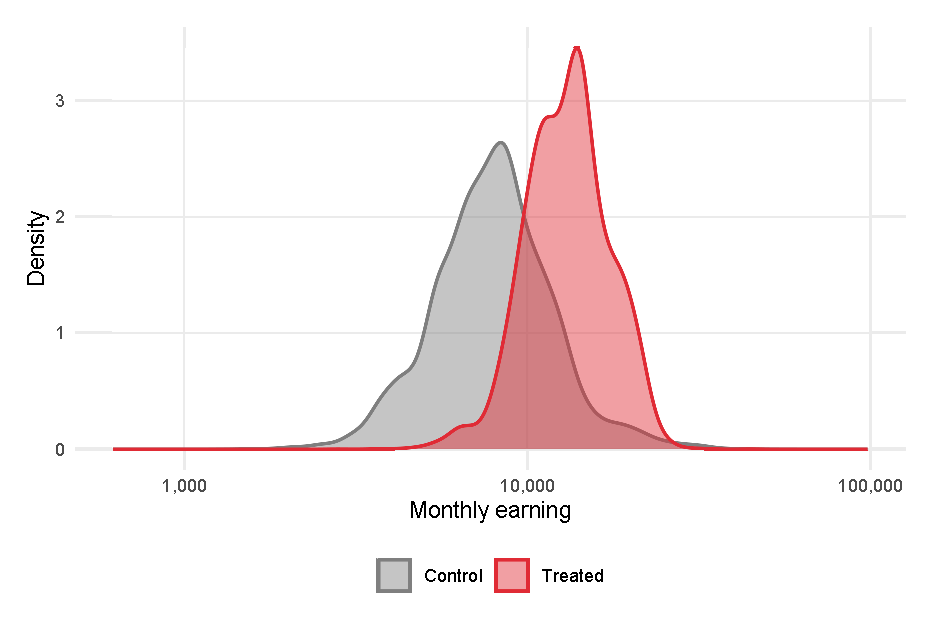
\includegraphics[width=\textwidth]{Figures/dist_wage_imp_alpha_human.eps}
    \caption{$\alpha$ human}
    \label{fig:dist_wage_imp_alpha_human}
  \end{subfigure}
  \hfill
  \begin{subfigure}[b]{0.49\textwidth}
    \centering
    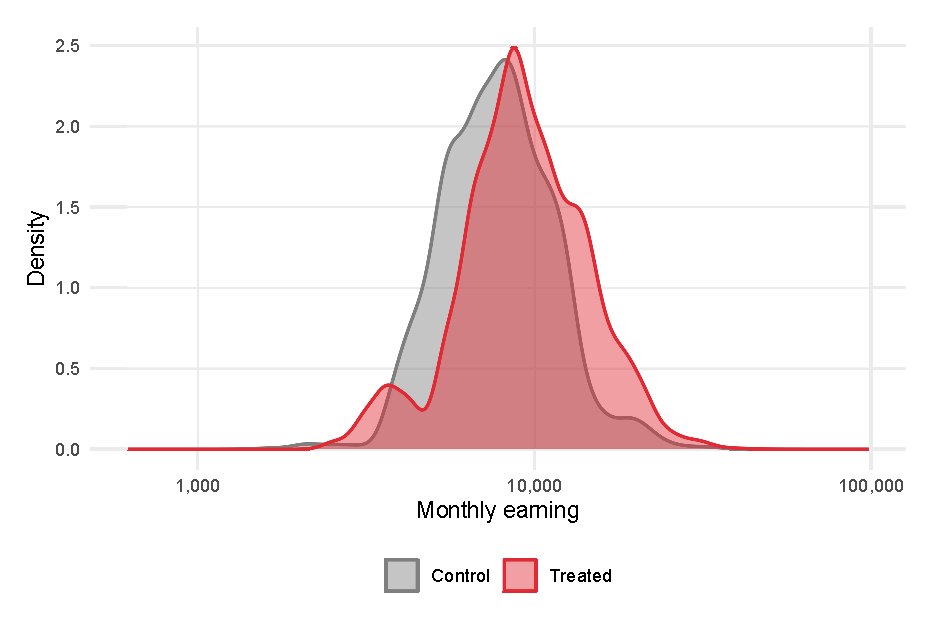
\includegraphics[width=\textwidth]{Figures/dist_wage_imp_beta_human.eps}
    \caption{$\beta$ human}
    \label{fig:dist_wage_imp_beta_human}
  \end{subfigure}
  \hfill
  \begin{subfigure}[b]{0.49\textwidth}
    \centering
    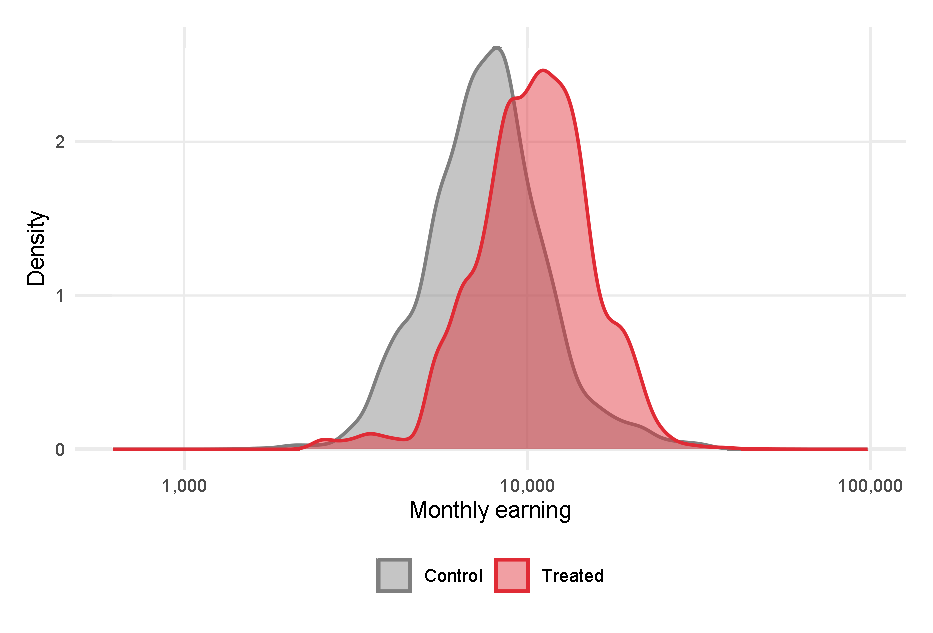
\includegraphics[width=\textwidth]{Figures/dist_wage_imp_alpha_gpt.eps}
    \caption{$\alpha$ GPT-4o}
    \label{fig:dist_wage_imp_alpha_gpt}
  \end{subfigure}
  \hfill
  \begin{subfigure}[b]{0.49\textwidth}
    \centering
    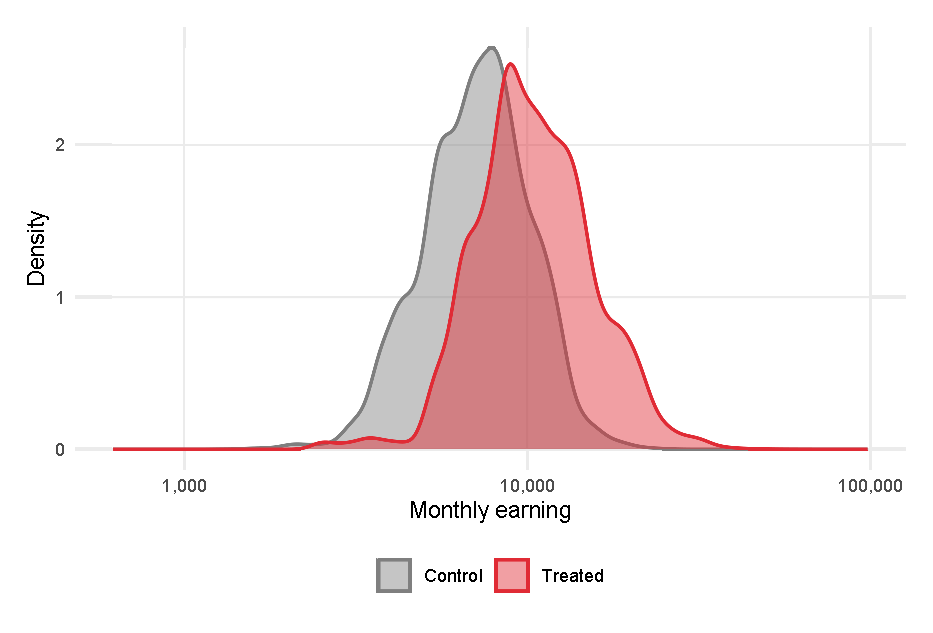
\includegraphics[width=\textwidth]{Figures/dist_wage_imp_beta_gpt.eps}
    \caption{$\beta$ GPT-4o}
    \label{fig:dist_wage_imp_beta_gpt}
  \end{subfigure}
  \hfill
  \label{fig:wage_dist}
  \begin{minipage}{0.6\textwidth}
    \small
    \textit{Note:} Kernel density of imputed monthly earnings (MXN, log scale), by treatment group, with weights by number of workers and averaged across the before and after treatment periods.
  \end{minipage}
\end{figure}

\begin{figure}[H]
  \centering
  \caption{Trends in monthly earnings by treatment group}
  \label{fig:trend_wage_imp}
  \begin{subfigure}[b]{0.49\textwidth}
    \centering
    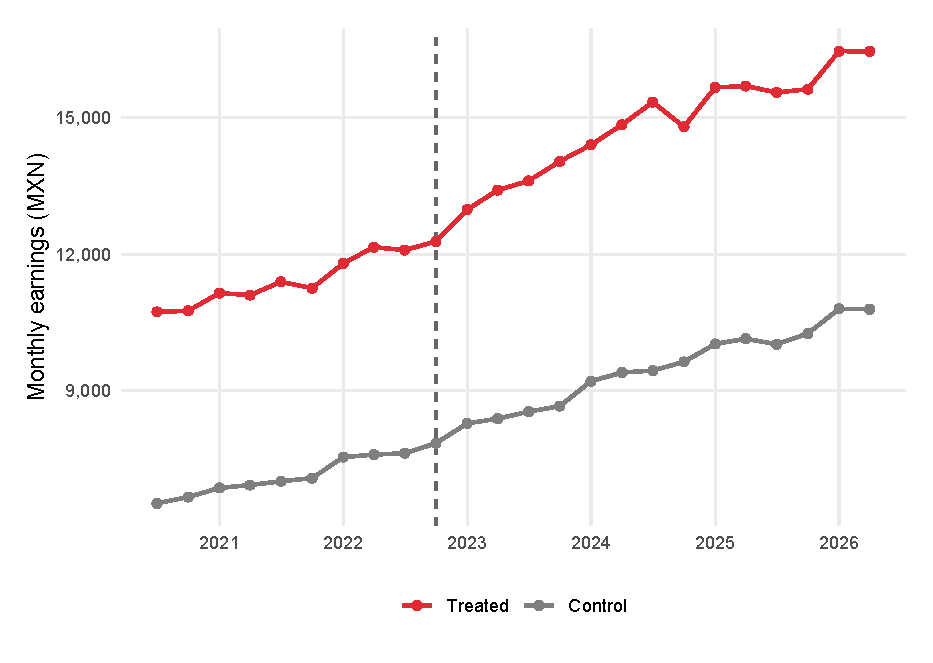
\includegraphics[width=\textwidth]{Figures/trend_wage_imp_alpha_human.eps}
    \caption{Human alpha}
    \label{fig:trend_wage_imp_human_alpha}
  \end{subfigure}
  \hfill
  \begin{subfigure}[b]{0.49\textwidth}
    \centering
    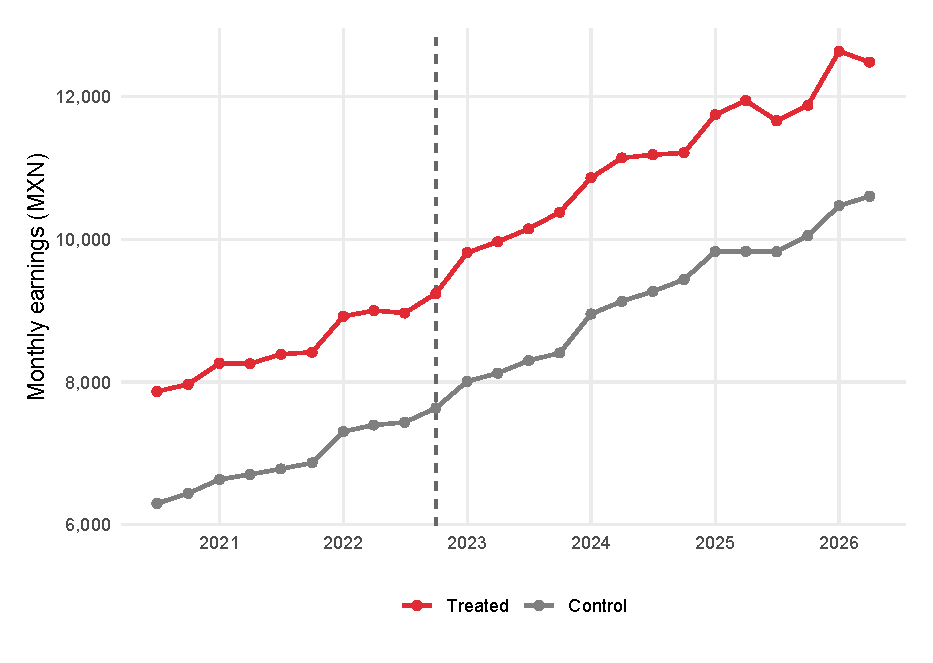
\includegraphics[width=\textwidth]{Figures/trend_wage_imp_beta_human.eps}
    \caption{Human beta}
    \label{fig:trend_wage_imp_beta_human}
  \end{subfigure}
  \hfill
  \begin{subfigure}[b]{0.49\textwidth}
    \centering
    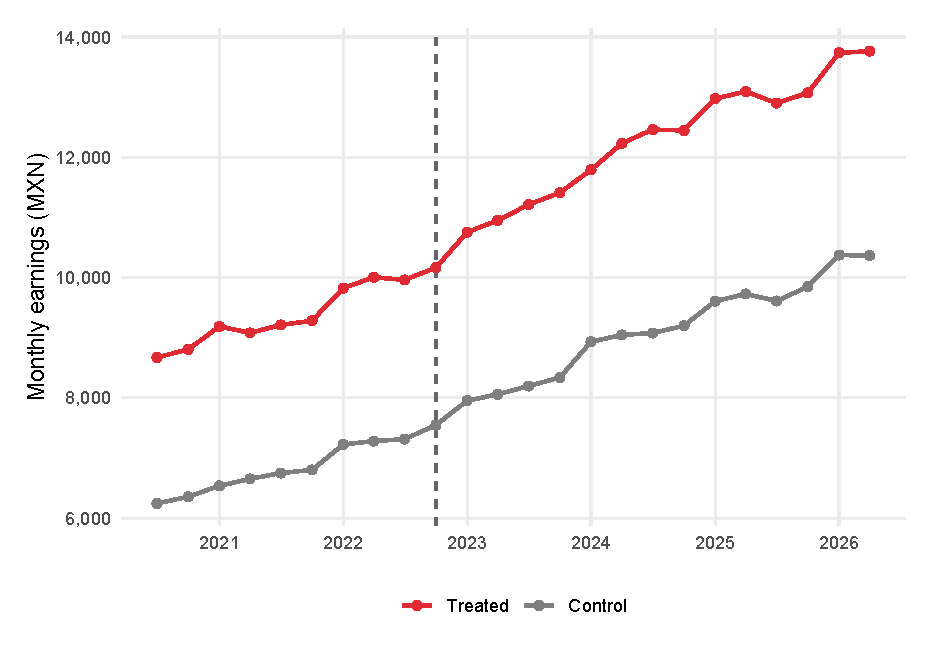
\includegraphics[width=\textwidth]{Figures/trend_wage_imp_alpha_gpt.eps}
    \caption{GPT-4o alpha}
    \label{fig:trend_wage_imp_gpt_alpha}
  \end{subfigure}
  \hfill
  \begin{subfigure}[b]{0.49\textwidth}
    \centering
    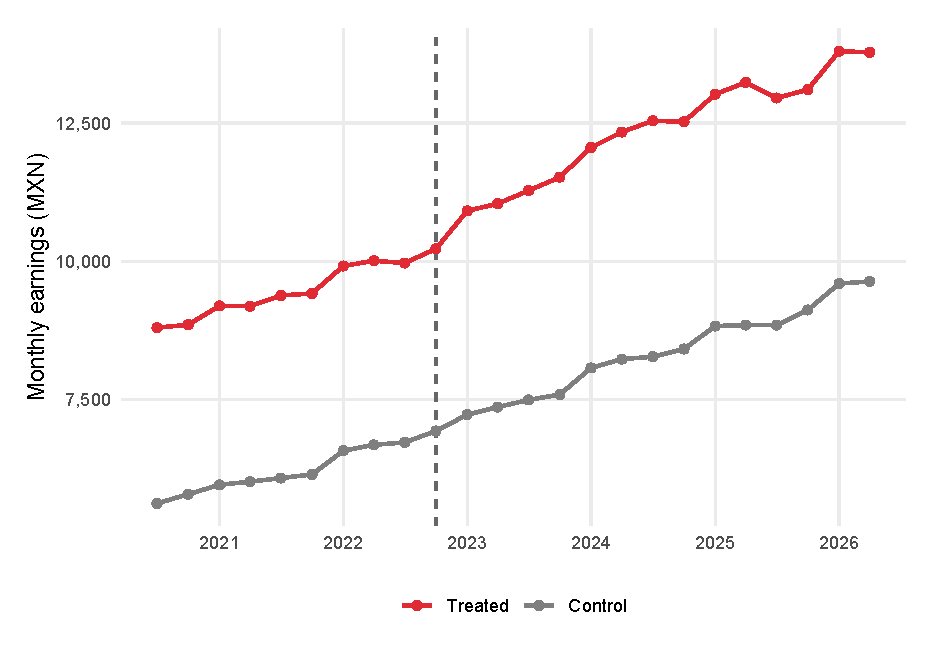
\includegraphics[width=\textwidth]{Figures/trend_wage_imp_beta_gpt.eps}
    \caption{GPT-4o beta}
    \label{fig:trend_wage_imp_gpt_beta}
  \end{subfigure}
  \hfill
  \begin{minipage}{\textwidth}
    \small
    \textit{Note:} The figure displays trends of monthly earnings in treated and control occupations over time. Panel (a) and (b) use the human exposure measure, while panel (c) and (d) use the GPT-4o exposure measure.
  \end{minipage}
\end{figure}

\begin{figure}[H]
  \centering
  \caption{Trends on the logarithm of the number of workers by treatment group}
  \label{fig:trend_workers_imp}
  \begin{subfigure}[b]{0.49\textwidth}
    \centering
    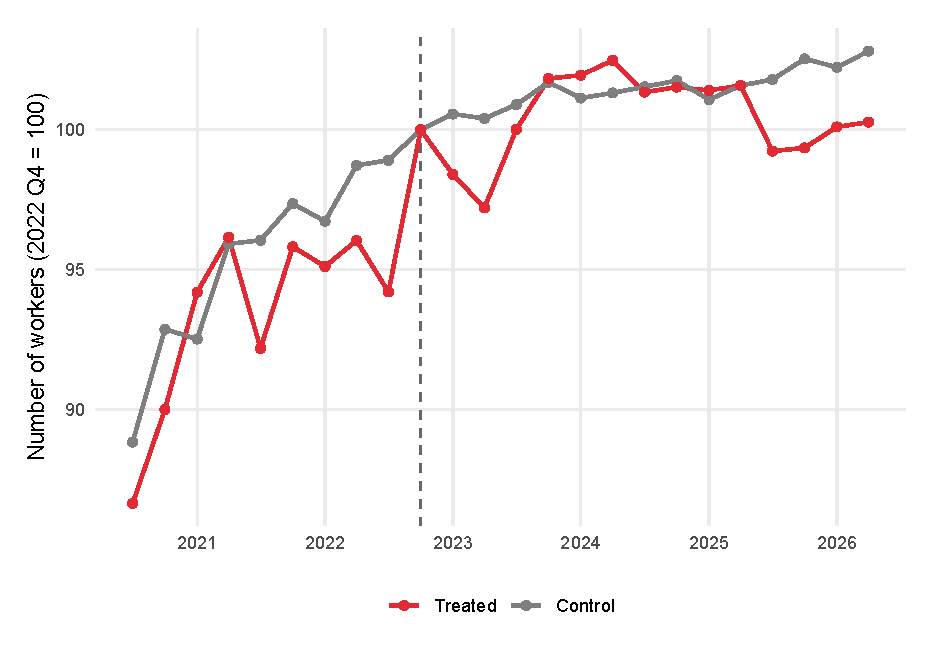
\includegraphics[width=\textwidth]{Figures/trend_n_pop_alpha_human.eps}
    \caption{Human alpha}
    \label{fig:trend_workers_imp_human_alpha}
  \end{subfigure}
  \hfill
  \begin{subfigure}[b]{0.49\textwidth}
    \centering
    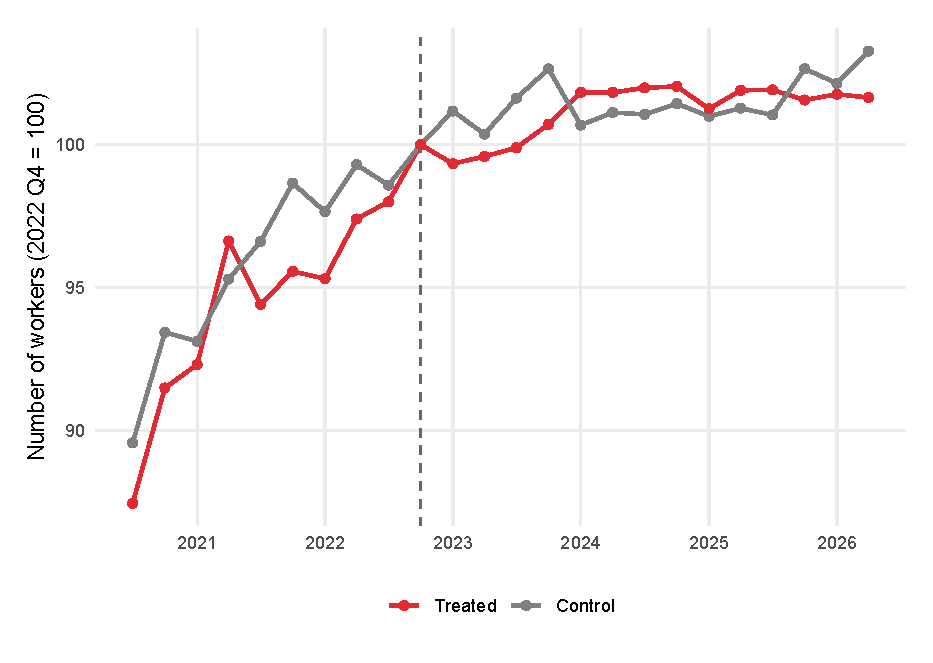
\includegraphics[width=\textwidth]{Figures/trend_n_pop_beta_human.eps}
    \caption{Human beta}
    \label{fig:trend_workers_imp_beta_human}
  \end{subfigure}
  \hfill
  \begin{subfigure}[b]{0.49\textwidth}
    \centering
    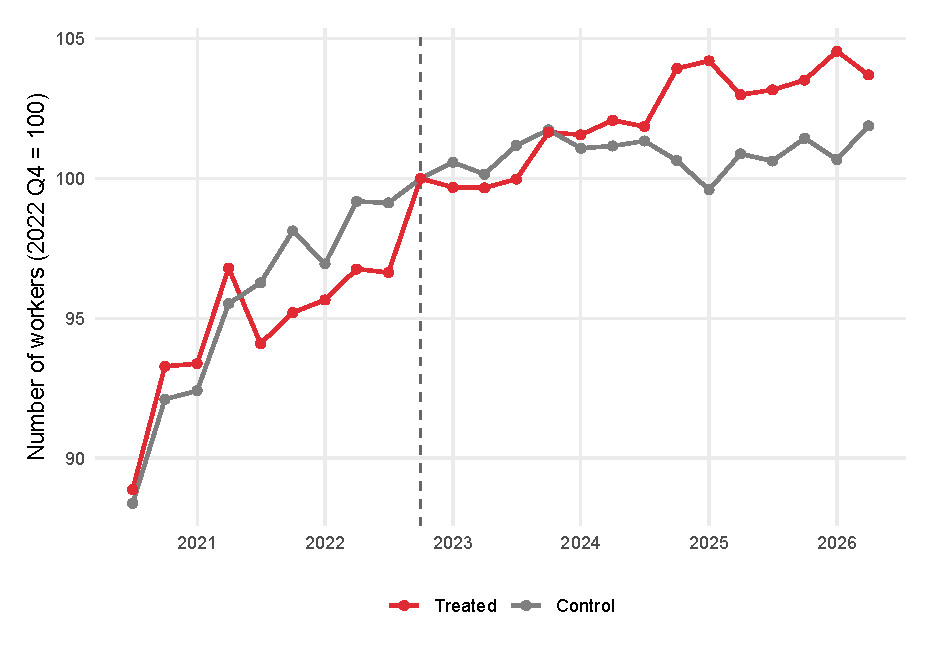
\includegraphics[width=\textwidth]{Figures/trend_n_pop_alpha_gpt.eps}
    \caption{GPT-4o alpha}
    \label{fig:trend_workers_imp_gpt_alpha}
  \end{subfigure}
  \hfill
  \begin{subfigure}[b]{0.49\textwidth}
    \centering
    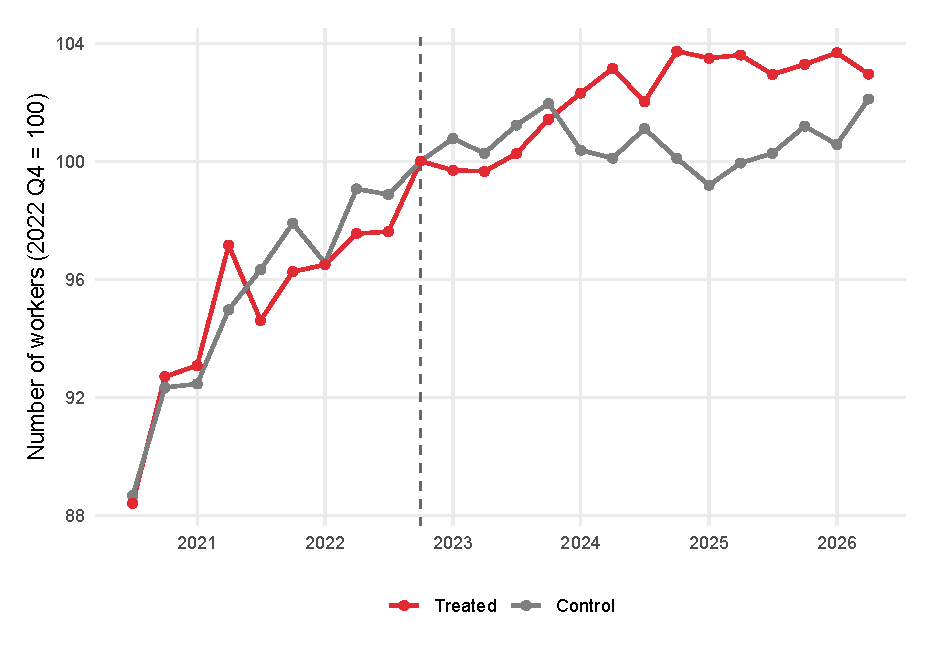
\includegraphics[width=\textwidth]{Figures/trend_n_pop_beta_gpt.eps}
    \caption{GPT-4o beta}
    \label{fig:trend_workers_imp_gpt_beta}
  \end{subfigure}
  \hfill
  \begin{minipage}{\textwidth}
    \small
    \textit{Note:} The figure displays trends for the number of workers in treated and control occupations over time. Panel (a) and (b) use the human exposure measure, while panel (c) and (d) use the GPT-4o exposure measure.
  \end{minipage}
\end{figure}

\begin{figure}[H]
  \centering
  \caption{Trends on the logarithm of the number of informal workers by treatment group}
  \label{fig:trend_informal_imp}
  \begin{subfigure}[b]{0.49\textwidth}
    \centering
    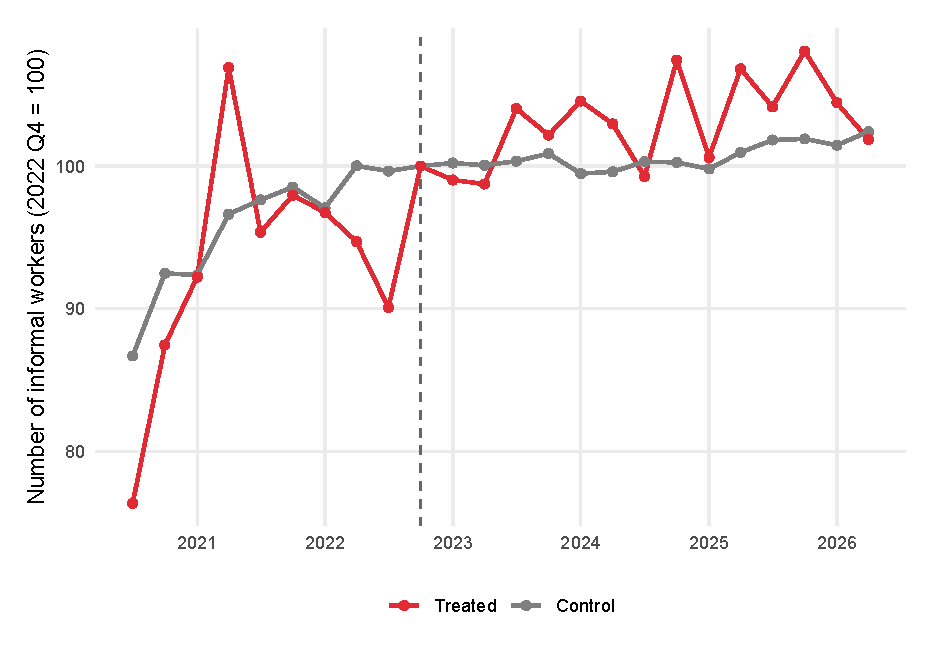
\includegraphics[width=\textwidth]{Figures/trend_informal_alpha_human.eps}
    \caption{Human alpha}
    \label{fig:trend_informal_imp_human_alpha}
  \end{subfigure}
  \hfill
  \begin{subfigure}[b]{0.49\textwidth}
    \centering
    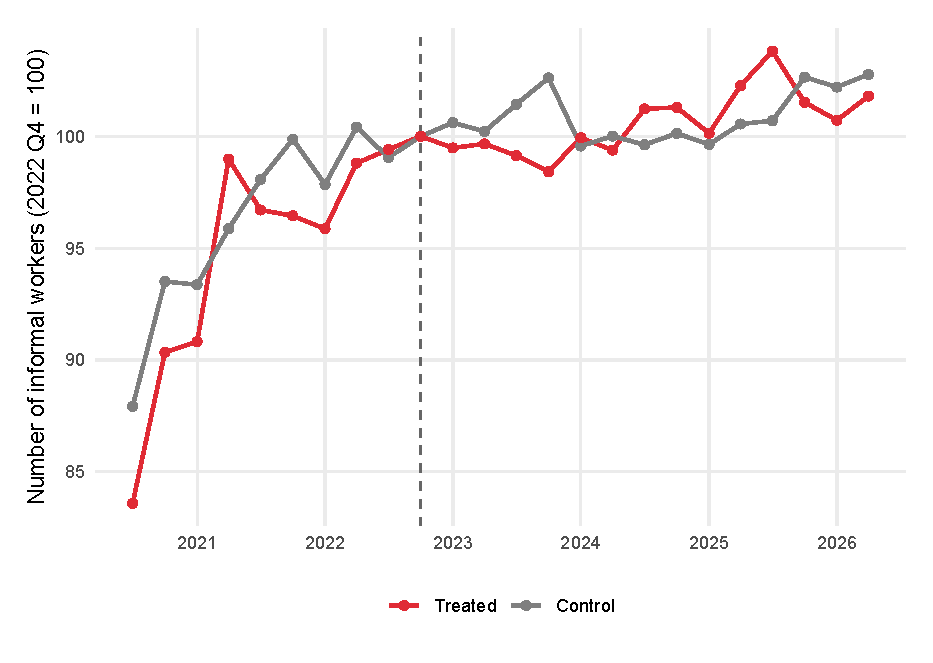
\includegraphics[width=\textwidth]{Figures/trend_informal_beta_human.eps}
    \caption{Human beta}
    \label{fig:trend_informal_imp_beta_human}
  \end{subfigure}
  \hfill
  \begin{subfigure}[b]{0.49\textwidth}
    \centering
    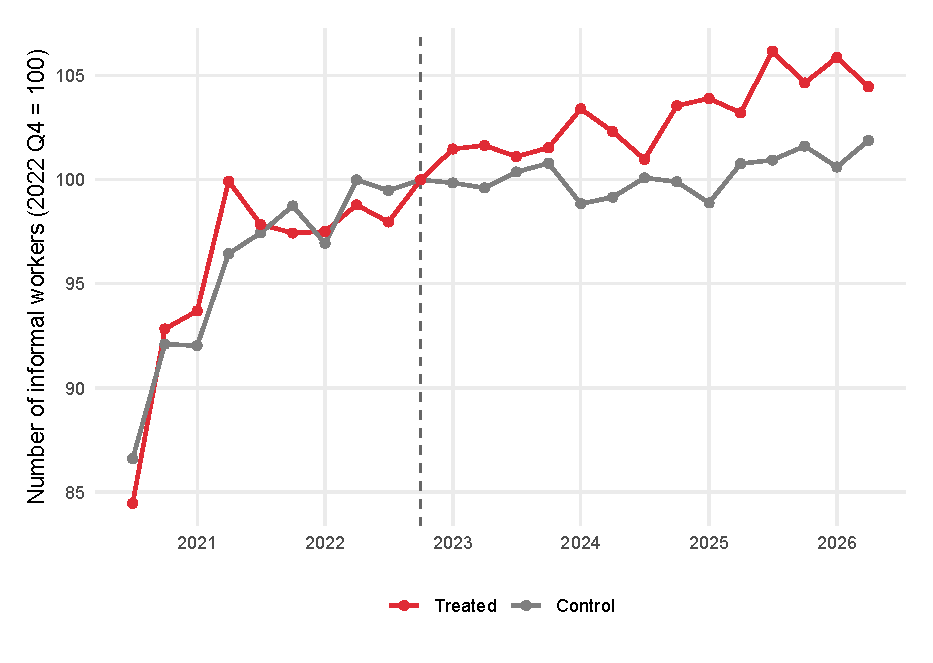
\includegraphics[width=\textwidth]{Figures/trend_informal_alpha_gpt.eps}
    \caption{GPT-4o alpha}
    \label{fig:trend_informal_imp_gpt_alpha}
  \end{subfigure}
  \hfill
  \begin{subfigure}[b]{0.49\textwidth}
    \centering
    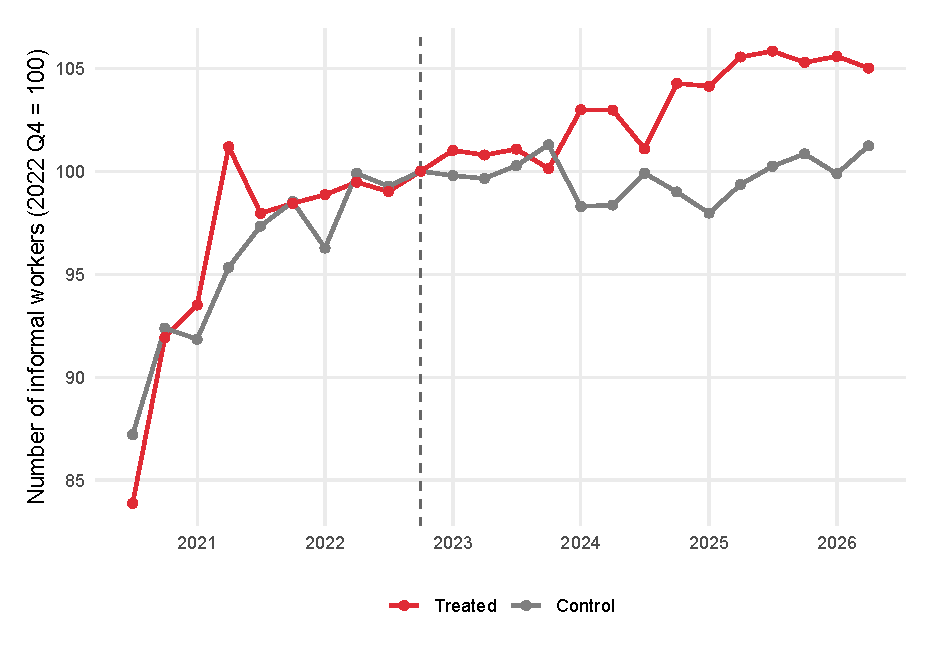
\includegraphics[width=\textwidth]{Figures/trend_informal_beta_gpt.eps}
    \caption{GPT-4o beta}
    \label{fig:trend_informal_imp_gpt_beta}
  \end{subfigure}
  \hfill
  \begin{minipage}{\textwidth}
    \small
    \textit{Note:} The figure displays trends for the number of informal workers in treated and control occupations over time. Panel (a) and (b) use the human exposure measure, while panel (c) and (d) use the GPT-4o exposure measure.
  \end{minipage}
\end{figure}




\begin{table}[H]
  \centering
  \caption{\label{tab:did_main}Difference in differences estimates: effect of ChatGPT's release on labor market outcomes}
  \centering
  \resizebox{\ifdim\width>\linewidth\linewidth\else\width\fi}{!}{
    \begin{threeparttable}
      \begin{tabular}[t]{lcccc}
        \toprule
                                       & Log number of workers & Log number of informal workers & Monthly earnings (MXN) & Share of imputed wages (\%) \\
        \midrule
        \addlinespace[0.3em]
        \multicolumn{5}{l}{\textbf{Panel A: Human exposure}}                                                                                           \\
        \addlinespace[0.3em]
        \multicolumn{5}{l}{\textit{Beta}}                                                                                                              \\
        \hspace{1em}Treated x Post     & 0.004                 & 0.042                          & 259.091                & 0.526                       \\
        \hspace{1em}                   & (0.023)               & (0.027)                        & (193.619)              & (0.346)                     \\
        \hspace{1em}Female (share)     & 0.107                 & 0.250**                        & -1103.525**            & -3.700**                    \\
        \hspace{1em}                   & (0.075)               & (0.118)                        & (533.885)              & (1.646)                     \\
        \hspace{1em}Years of schooling & 0.002                 & -0.024                         & 155.285***             & 0.808***                    \\
        \hspace{1em}                   & (0.008)               & (0.016)                        & (38.079)               & (0.157)                     \\
        \hspace{1em}Age (years)        & -0.011**              & -0.018***                      & 10.462                 & 0.190***                    \\
        \hspace{1em}                   & (0.006)               & (0.005)                        & (19.250)               & (0.067)                     \\
        \addlinespace[0.3em]
        \multicolumn{5}{l}{\textit{Alpha}}                                                                                                             \\
        \hspace{1em}Treated x Post     & -0.006                & 0.072*                         & 1011.201***            & -0.290                      \\
        \hspace{1em}                   & (0.040)               & (0.038)                        & (191.886)              & (0.415)                     \\
        \hspace{1em}Female (share)     & 0.109                 & 0.255**                        & -1116.064**            & -3.559**                    \\
        \hspace{1em}                   & (0.075)               & (0.119)                        & (500.374)              & (1.666)                     \\
        \hspace{1em}Years of schooling & 0.002                 & -0.023                         & 174.504***             & 0.786***                    \\
        \hspace{1em}                   & (0.007)               & (0.016)                        & (38.070)               & (0.155)                     \\
        \hspace{1em}Age (years)        & -0.011*               & -0.018***                      & 17.331                 & 0.184***                    \\
        \hspace{1em}                   & (0.006)               & (0.005)                        & (18.755)               & (0.067)                     \\
        \addlinespace[0.3em]
        \multicolumn{5}{l}{\textbf{Panel B: GPT-4o exposure}}                                                                                          \\
        \addlinespace[0.3em]
        \multicolumn{5}{l}{\textit{Alpha}}                                                                                                             \\
        \hspace{1em}Treated x Post     & 0.016                 & 0.056**                        & 625.079***             & 0.427                       \\
        \hspace{1em}                   & (0.024)               & (0.026)                        & (218.555)              & (0.344)                     \\
        \hspace{1em}Female (share)     & 0.105                 & 0.248**                        & -1182.879**            & -3.674**                    \\
        \hspace{1em}                   & (0.074)               & (0.117)                        & (523.082)              & (1.655)                     \\
        \hspace{1em}Years of schooling & 0.002                 & -0.023                         & 162.929***             & 0.804***                    \\
        \hspace{1em}                   & (0.008)               & (0.016)                        & (38.205)               & (0.156)                     \\
        \hspace{1em}Age (years)        & -0.011*               & -0.018***                      & 12.240                 & 0.189***                    \\
        \hspace{1em}                   & (0.006)               & (0.005)                        & (18.899)               & (0.067)                     \\
        \addlinespace[0.3em]
        \multicolumn{5}{l}{\textit{Beta}}                                                                                                              \\
        \hspace{1em}Treated x Post     & 0.013                 & 0.055**                        & 750.381***             & 0.610*                      \\
        \hspace{1em}                   & (0.022)               & (0.025)                        & (200.314)              & (0.333)                     \\
        \hspace{1em}Female (share)     & 0.106                 & 0.251**                        & -1162.391**            & -3.676**                    \\
        \hspace{1em}                   & (0.075)               & (0.117)                        & (529.160)              & (1.650)                     \\
        \hspace{1em}Years of schooling & 0.002                 & -0.023                         & 166.153***             & 0.808***                    \\
        \hspace{1em}                   & (0.008)               & (0.016)                        & (38.305)               & (0.156)                     \\
        \hspace{1em}Age (years)        & -0.011*               & -0.018***                      & 15.279                 & 0.192***                    \\
        \hspace{1em}                   & (0.006)               & (0.005)                        & (18.315)               & (0.067)                     \\
        \bottomrule
      \end{tabular}
      \begin{tablenotes}
        \item \textit{Note:} Each column is a separate regression of the outcome on $\text{Post}_{t=2022q4} \times \text{ExposureGPT}_j$, plus the ratio of female workers, average years of schooling and average age of the occupation, with occupation and quarter fixed effects. Observations are weighted by occupation size measured as the number of workers. Standard errors clustered by occupation in parentheses. Treated occupations are defined by the median exposure measure of interest. $* p<0.10, ** p<0.05, *** p<0.01$
      \end{tablenotes}
    \end{threeparttable}}
\end{table}




\begin{figure}[H]
  \centering
  \caption{Impact of ChatGPT's release on monthly earnings}
  \label{fig:es_monthly_earnings}

  \begin{subfigure}[b]{0.7\textwidth}
    \centering
    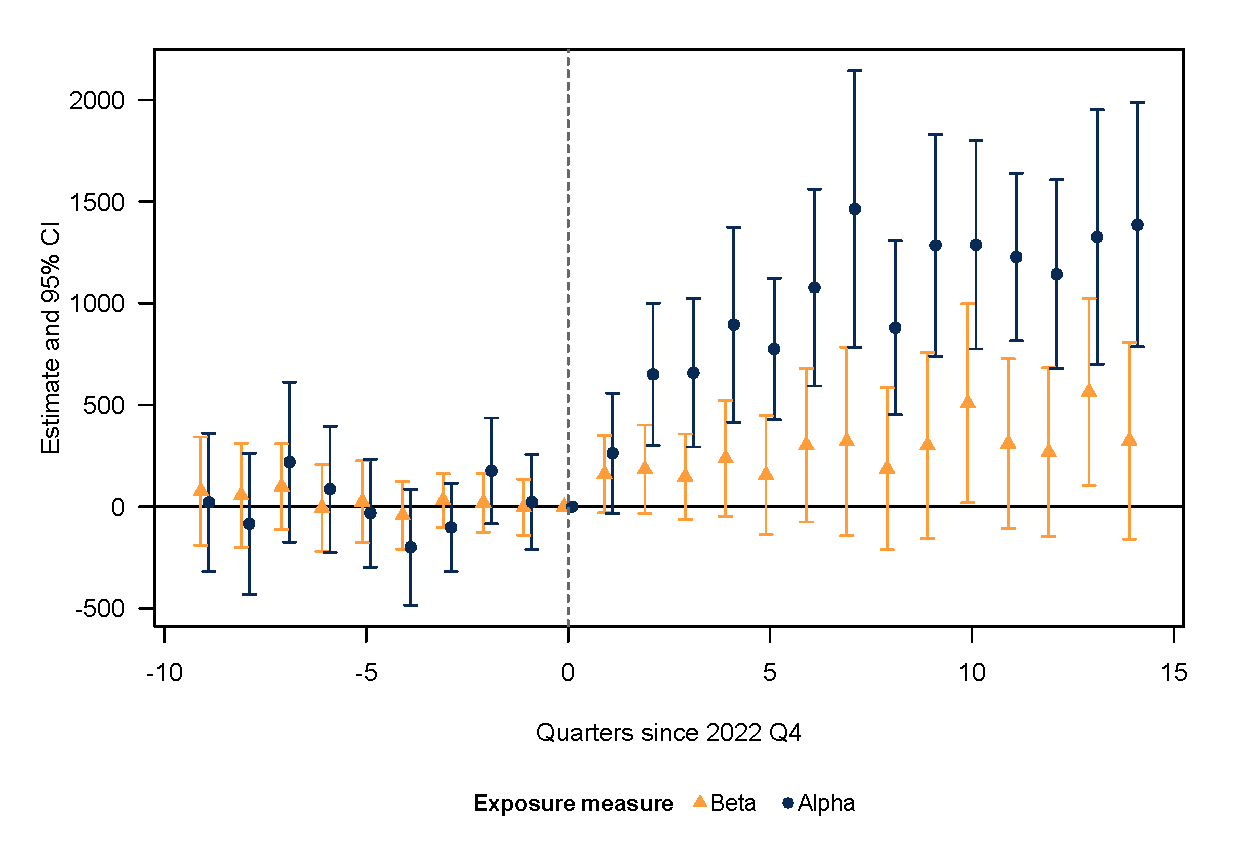
\includegraphics[width=\textwidth]{Figures/es_wage_imp_human.eps}
    \caption{Monthly earnings Human}
    \label{fig:es_wage_imp_human}
  \end{subfigure}

  \medskip

  \begin{subfigure}[b]{0.7\textwidth}
    \centering
    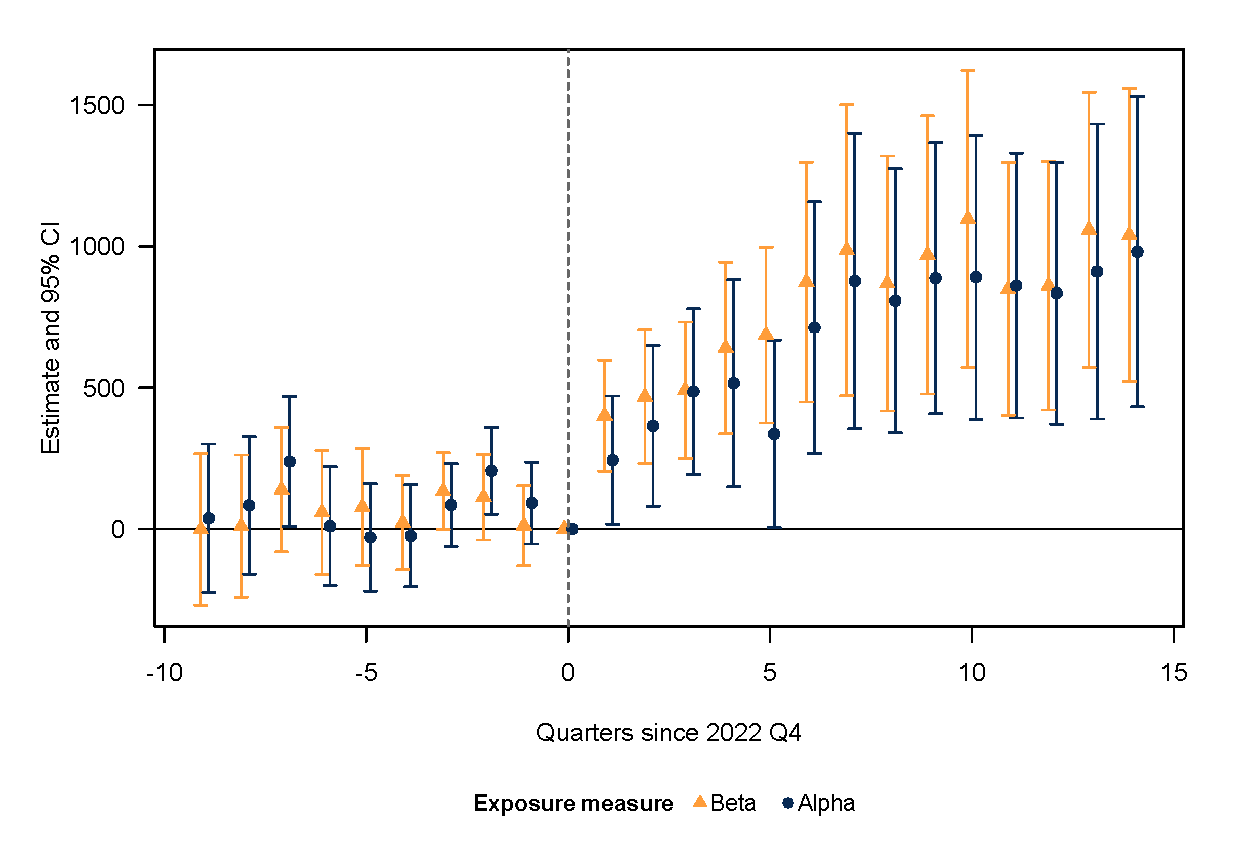
\includegraphics[width=\textwidth]{Figures/es_wage_imp_gpt.eps}
    \caption{Monthly earnings GPT-4o}
    \label{fig:es_wage_imp_gpt}
  \end{subfigure}

  \medskip

  \begin{minipage}{\textwidth}
    \small
    \textit{Note:} The figure shows the main results from my event study analysis (see \cref{ES}). Both panels show the effect on the average monthly earnings of the treated occupations relative to the control occupations over time. Panel (a) uses the human exposure measure, while panel (b) uses the GPT-4o exposure measure. Monthly earnings include observed and imputed values (PMM).
  \end{minipage}
\end{figure}

\begin{figure}[H]
  \centering
  \caption{Impact of ChatGPT's release on the number of workers}
  \label{fig:es_log_emp}

  \begin{subfigure}[b]{0.7\textwidth}
    \centering
    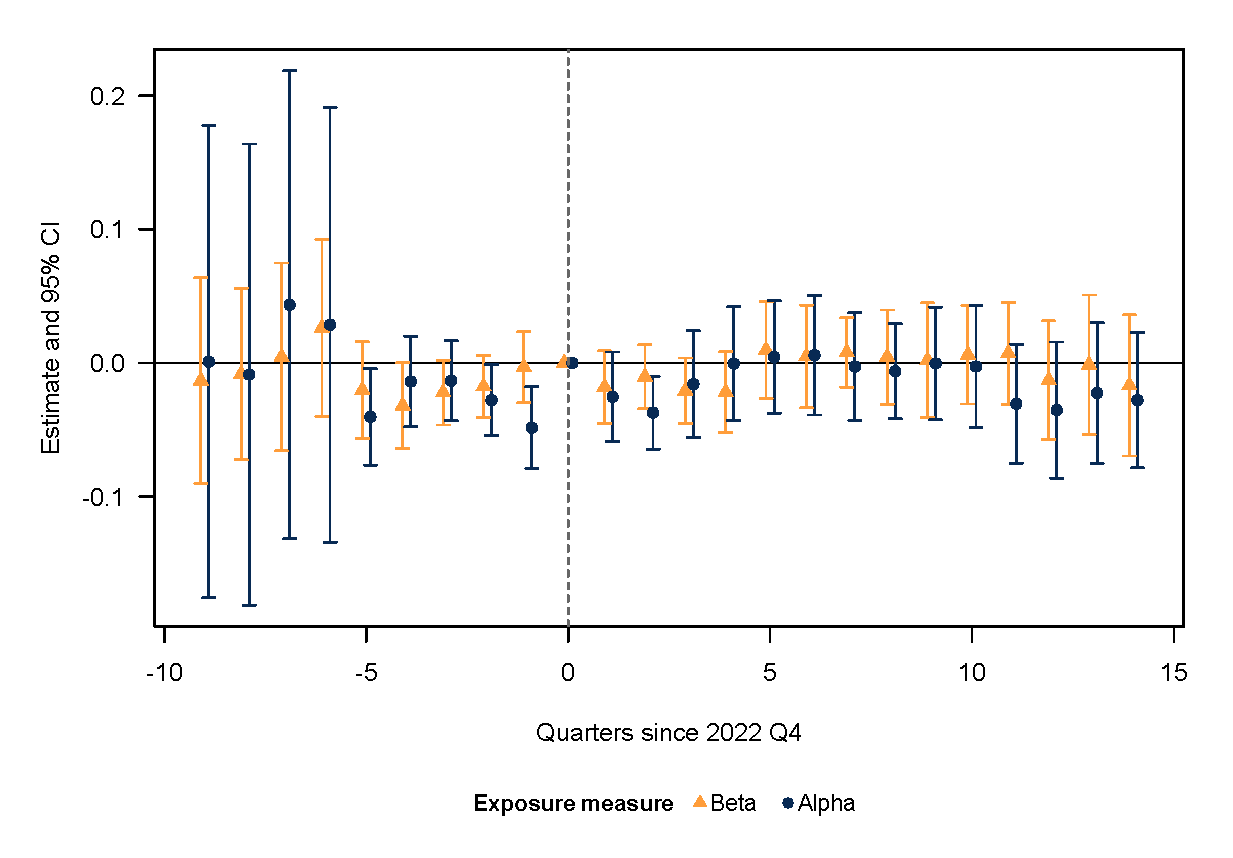
\includegraphics[width=\textwidth]{Figures/es_log_emp_human.eps}
    \caption{Number of workers Human}
    \label{fig:es_log_emp_human}
  \end{subfigure}

  \medskip

  \begin{subfigure}[b]{0.7\textwidth}
    \centering
    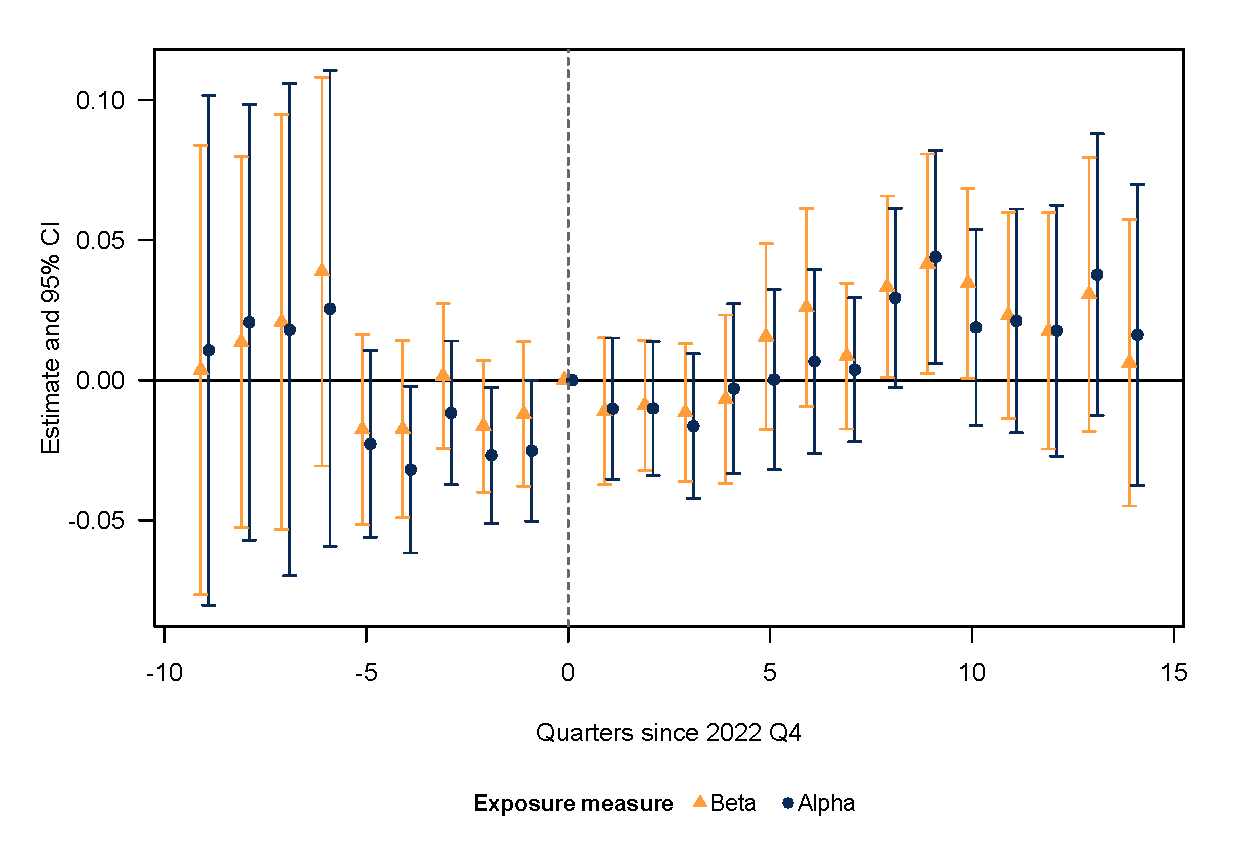
\includegraphics[width=\textwidth]{Figures/es_log_emp_gpt.eps}
    \caption{Number of workers GPT-4o}
    \label{fig:es_log_emp_gpt}
  \end{subfigure}

  \medskip

  \begin{minipage}{\textwidth}
    \small
    \textit{Note:} The figure shows the main results from my event study analysis (see \cref{ES}). Both panels show the effect on the logarithm of the average number of workers of the treated occupations relative to the control occupations over time. Panel (a) uses the human exposure measure, while panel (b) uses the GPT-4o exposure measure.
  \end{minipage}
\end{figure}

\begin{figure}[H]
  \centering
  \caption{Impact of ChatGPT's release on the number of informal workers}
  \label{fig:es_log_informal}

  \begin{subfigure}[b]{0.7\textwidth}
    \centering
    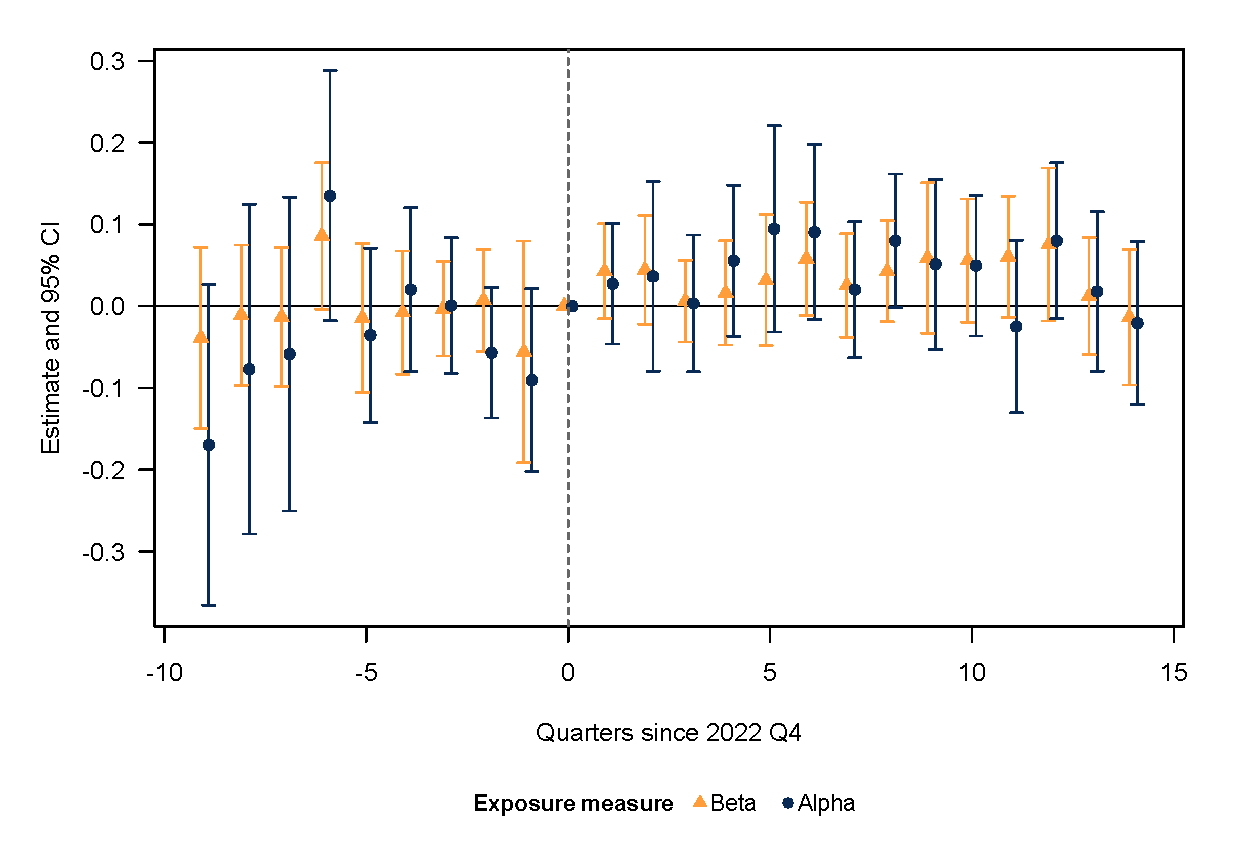
\includegraphics[width=\textwidth]{Figures/es_log_informal_human.eps}
    \caption{Number of informal workers Human}
    \label{fig:es_log_informal_human}
  \end{subfigure}

  \medskip

  \begin{subfigure}[b]{0.7\textwidth}
    \centering
    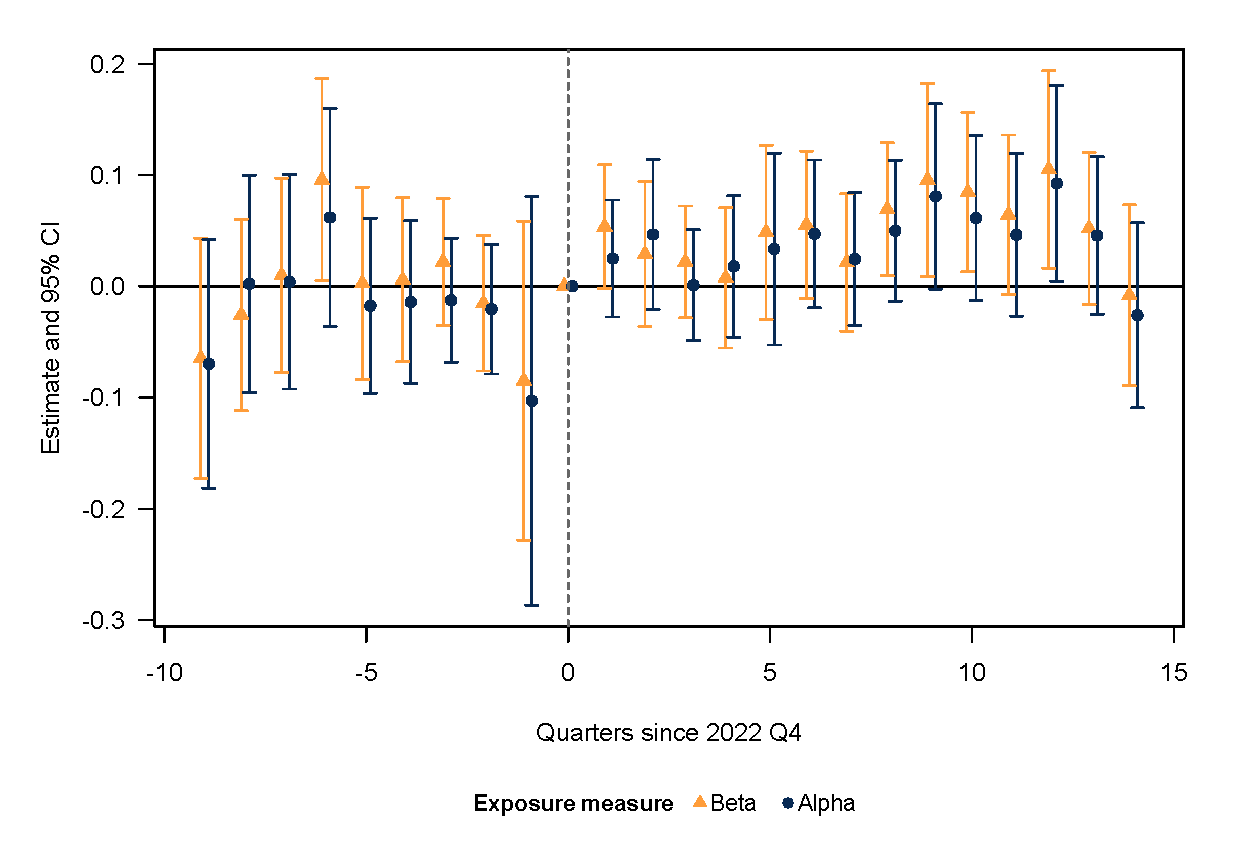
\includegraphics[width=\textwidth]{Figures/es_log_informal_gpt.eps}
    \caption{Number of informal workers GPT-4o}
    \label{fig:es_log_informal_gpt}
  \end{subfigure}

  \medskip

  \begin{minipage}{\textwidth}
    \small
    \textit{Note:} The figure shows the main results from my event study analysis (see \cref{ES}). Both panels show the effect on the logarithm of the average number of informal workers of the treated occupations relative to the control occupations over time. Panel (a) uses the human exposure measure, while panel (b) uses the GPT-4o exposure measure.
  \end{minipage}
\end{figure}

\begingroup
\footnotesize
\renewcommand{\arraystretch}{0.9}
\setlength{\tabcolsep}{4pt}
\begin{longtable}{lcccc}
  \caption{\label{tab:es_wage_imp} Monthly earnings (MXN): event study estimates (ref. = 2022 Q4)}                             \\
  \toprule
                                  & \multicolumn{4}{c}{monthly earnings}                                                       \\
                                  & Human Beta                           & Human Alpha     & GPT-4o Beta     & GPT-4o Alpha    \\
                                  & (1)                                  & (2)             & (3)             & (4)             \\
  \midrule
  \endfirsthead
  \multicolumn{5}{l}{\textit{Table \thetable\ (continued)}}                                                                    \\
  \toprule
                                  & \multicolumn{4}{c}{wage\_imp}                                                              \\
                                  & Human Beta                           & Human Alpha     & GPT-4o Beta     & GPT-4o Alpha    \\
                                  & (1)                                  & (2)             & (3)             & (4)             \\
  \midrule
  \endhead
  \midrule
  \multicolumn{5}{r}{\textit{Continued on next page}}                                                                          \\
  \endfoot
  \bottomrule
  \endlastfoot
  Treated $\times$ Quarter $=$ -9 & 76.7                                 & 20.9            & -1.84           & 38.0            \\
                                  & (135.3)                              & (173.0)         & (136.2)         & (133.7)         \\
  Treated $\times$ Quarter $=$ -8 & 56.0                                 & -84.2           & 9.86            & 83.7            \\
                                  & (129.7)                              & (176.5)         & (128.2)         & (123.7)         \\
  Treated $\times$ Quarter $=$ -7 & 98.4                                 & 219.1           & 139.0           & 238.7$^{**}$    \\
                                  & (107.0)                              & (200.1)         & (111.9)         & (116.9)         \\
  Treated $\times$ Quarter $=$ -6 & -5.91                                & 86.0            & 58.5            & 9.76            \\
                                  & (109.0)                              & (157.8)         & (111.2)         & (107.1)         \\
  Treated $\times$ Quarter $=$ -5 & 23.7                                 & -32.1           & 77.6            & -29.9           \\
                                  & (102.4)                              & (135.1)         & (105.4)         & (96.6)          \\
  Treated $\times$ Quarter $=$ -4 & -42.7                                & -199.2          & 22.6            & -24.3           \\
                                  & (84.6)                               & (145.0)         & (84.7)          & (91.9)          \\
  Treated $\times$ Quarter $=$ -3 & 30.2                                 & -102.0          & 133.5$^{*}$     & 84.7            \\
                                  & (66.8)                               & (110.2)         & (69.1)          & (74.7)          \\
  Treated $\times$ Quarter $=$ -2 & 19.3                                 & 175.7           & 112.4           & 206.1$^{***}$   \\
                                  & (73.7)                               & (132.4)         & (76.8)          & (78.1)          \\
  Treated $\times$ Quarter $=$ -1 & -3.22                                & 22.8            & 11.7            & 91.9            \\
                                  & (70.2)                               & (118.7)         & (72.0)          & (73.7)          \\
  Treated $\times$ Quarter $=$ 1  & 160.1$^{*}$                          & 262.3$^{*}$     & 400.9$^{***}$   & 243.7$^{**}$    \\
                                  & (96.9)                               & (150.4)         & (99.9)          & (115.4)         \\
  Treated $\times$ Quarter $=$ 2  & 184.0$^{*}$                          & 650.5$^{***}$   & 468.1$^{***}$   & 365.3$^{**}$    \\
                                  & (110.7)                              & (178.1)         & (120.5)         & (144.6)         \\
  Treated $\times$ Quarter $=$ 3  & 146.9                                & 658.2$^{***}$   & 491.4$^{***}$   & 486.3$^{***}$   \\
                                  & (106.9)                              & (185.7)         & (122.8)         & (149.0)         \\
  Treated $\times$ Quarter $=$ 4  & 236.3                                & 894.6$^{***}$   & 640.4$^{***}$   & 515.9$^{***}$   \\
                                  & (144.9)                              & (244.1)         & (154.4)         & (186.4)         \\
  Treated $\times$ Quarter $=$ 5  & 155.4                                & 774.8$^{***}$   & 686.2$^{***}$   & 336.2$^{**}$    \\
                                  & (148.1)                              & (177.2)         & (158.2)         & (168.6)         \\
  Treated $\times$ Quarter $=$ 6  & 302.1                                & 1,077.0$^{***}$ & 873.6$^{***}$   & 712.7$^{***}$   \\
                                  & (192.2)                              & (246.1)         & (215.8)         & (226.5)         \\
  Treated $\times$ Quarter $=$ 7  & 319.9                                & 1,463.4$^{***}$ & 986.3$^{***}$   & 877.8$^{***}$   \\
                                  & (235.7)                              & (345.9)         & (261.7)         & (265.9)         \\
  Treated $\times$ Quarter $=$ 8  & 186.6                                & 879.4$^{***}$   & 868.6$^{***}$   & 807.5$^{***}$   \\
                                  & (203.0)                              & (217.3)         & (229.5)         & (237.8)         \\
  Treated $\times$ Quarter $=$ 9  & 301.3                                & 1,284.2$^{***}$ & 969.8$^{***}$   & 887.3$^{***}$   \\
                                  & (232.9)                              & (277.2)         & (250.4)         & (244.0)         \\
  Treated $\times$ Quarter $=$ 10 & 508.3$^{**}$                         & 1,287.4$^{***}$ & 1,097.0$^{***}$ & 891.0$^{***}$   \\
                                  & (248.8)                              & (260.5)         & (267.0)         & (255.5)         \\
  Treated $\times$ Quarter $=$ 11 & 309.5                                & 1,227.3$^{***}$ & 849.4$^{***}$   & 861.5$^{***}$   \\
                                  & (212.2)                              & (209.8)         & (227.5)         & (238.4)         \\
  Treated $\times$ Quarter $=$ 12 & 267.9                                & 1,142.9$^{***}$ & 860.6$^{***}$   & 834.6$^{***}$   \\
                                  & (210.9)                              & (236.1)         & (223.5)         & (235.9)         \\
  Treated $\times$ Quarter $=$ 13 & 564.0$^{**}$                         & 1,325.9$^{***}$ & 1,058.6$^{***}$ & 911.2$^{***}$   \\
                                  & (233.9)                              & (318.4)         & (247.8)         & (265.5)         \\
  Treated $\times$ Quarter $=$ 14 & 324.2                                & 1,385.9$^{***}$ & 1,040.3$^{***}$ & 981.3$^{***}$   \\
                                  & (246.2)                              & (305.3)         & (263.4)         & (279.2)         \\
  female                          & -1,123.5$^{**}$                      & -1,184.2$^{**}$ & -1,237.5$^{**}$ & -1,278.9$^{**}$ \\
                                  & (531.2)                              & (493.7)         & (529.3)         & (517.6)         \\
  anios\_esc                      & 160.8$^{***}$                        & 187.1$^{***}$   & 174.6$^{***}$   & 173.4$^{***}$   \\
                                  & (38.0)                               & (38.5)          & (39.5)          & (38.2)          \\
  eda                             & 10.3                                 & 18.0            & 15.6            & 11.6            \\
                                  & (19.3)                               & (18.7)          & (18.2)          & (18.8)          \\
  \\
  Observations                    & 10,126                               & 10,126          & 10,126          & 10,126          \\
  R$^2$                           & 0.94962                              & 0.95125         & 0.95160         & 0.95092         \\
  \\
  occupation fixed effects        & $\checkmark$                         & $\checkmark$    & $\checkmark$    & $\checkmark$    \\
  period\_q fixed effects         & $\checkmark$                         & $\checkmark$    & $\checkmark$    & $\checkmark$    \\
\end{longtable}
\vspace{-1.5em}
\textit{Note: } Standard errors clustered by occupation. Occupation and quarter fixed effects included, weighted by number of workers per occupation
\endgroup

\newpage

\begingroup
\footnotesize
\renewcommand{\arraystretch}{0.9}
\setlength{\tabcolsep}{4pt}
\begin{longtable}{lcccc}
  \caption{\label{tab:es_log_emp} Log number of workers: event study estimates (ref. = 2022 Q4)}                              \\
  \toprule
                                  & \multicolumn{4}{c}{log number of workers}                                                 \\
                                  & Human Beta                                & Human Alpha    & GPT-4o Beta  & GPT-4o Alpha  \\
                                  & (1)                                       & (2)            & (3)          & (4)           \\
  \midrule
  \endfirsthead
  \multicolumn{5}{l}{\textit{Table \thetable\ (continued)}}                                                                   \\
  \toprule
                                  & \multicolumn{4}{c}{log\_emp}                                                              \\
                                  & Human Beta                                & Human Alpha    & GPT-4o Beta  & GPT-4o Alpha  \\
                                  & (1)                                       & (2)            & (3)          & (4)           \\
  \midrule
  \endhead
  \midrule
  \multicolumn{5}{r}{\textit{Continued on next page}}                                                                         \\
  \endfoot
  \bottomrule
  \endlastfoot
  Treated $\times$ Quarter $=$ -9 & -0.013                                    & 0.0009         & 0.004        & 0.011         \\
                                  & (0.039)                                   & (0.090)        & (0.041)      & (0.046)       \\
  Treated $\times$ Quarter $=$ -8 & -0.008                                    & -0.009         & 0.013        & 0.021         \\
                                  & (0.033)                                   & (0.088)        & (0.034)      & (0.040)       \\
  Treated $\times$ Quarter $=$ -7 & 0.004                                     & 0.044          & 0.021        & 0.018         \\
                                  & (0.036)                                   & (0.089)        & (0.038)      & (0.045)       \\
  Treated $\times$ Quarter $=$ -6 & 0.026                                     & 0.029          & 0.039        & 0.025         \\
                                  & (0.034)                                   & (0.083)        & (0.035)      & (0.043)       \\
  Treated $\times$ Quarter $=$ -5 & -0.020                                    & -0.040$^{**}$  & -0.018       & -0.023        \\
                                  & (0.018)                                   & (0.018)        & (0.017)      & (0.017)       \\
  Treated $\times$ Quarter $=$ -4 & -0.032$^{*}$                              & -0.014         & -0.017       & -0.032$^{**}$ \\
                                  & (0.016)                                   & (0.017)        & (0.016)      & (0.015)       \\
  Treated $\times$ Quarter $=$ -3 & -0.022$^{*}$                              & -0.013         & 0.002        & -0.012        \\
                                  & (0.012)                                   & (0.015)        & (0.013)      & (0.013)       \\
  Treated $\times$ Quarter $=$ -2 & -0.018                                    & -0.028$^{**}$  & -0.016       & -0.027$^{**}$ \\
                                  & (0.012)                                   & (0.013)        & (0.012)      & (0.012)       \\
  Treated $\times$ Quarter $=$ -1 & -0.003                                    & -0.048$^{***}$ & -0.012       & -0.025$^{*}$  \\
                                  & (0.013)                                   & (0.015)        & (0.013)      & (0.013)       \\
  Treated $\times$ Quarter $=$ 1  & -0.018                                    & -0.025         & -0.011       & -0.010        \\
                                  & (0.014)                                   & (0.017)        & (0.013)      & (0.013)       \\
  Treated $\times$ Quarter $=$ 2  & -0.010                                    & -0.037$^{***}$ & -0.009       & -0.010        \\
                                  & (0.012)                                   & (0.014)        & (0.012)      & (0.012)       \\
  Treated $\times$ Quarter $=$ 3  & -0.021$^{*}$                              & -0.016         & -0.012       & -0.016        \\
                                  & (0.012)                                   & (0.020)        & (0.012)      & (0.013)       \\
  Treated $\times$ Quarter $=$ 4  & -0.022                                    & -0.0005        & -0.007       & -0.003        \\
                                  & (0.015)                                   & (0.022)        & (0.015)      & (0.015)       \\
  Treated $\times$ Quarter $=$ 5  & 0.010                                     & 0.004          & 0.015        & 0.0002        \\
                                  & (0.018)                                   & (0.021)        & (0.017)      & (0.016)       \\
  Treated $\times$ Quarter $=$ 6  & 0.005                                     & 0.006          & 0.026        & 0.007         \\
                                  & (0.020)                                   & (0.023)        & (0.018)      & (0.017)       \\
  Treated $\times$ Quarter $=$ 7  & 0.008                                     & -0.003         & 0.009        & 0.004         \\
                                  & (0.013)                                   & (0.020)        & (0.013)      & (0.013)       \\
  Treated $\times$ Quarter $=$ 8  & 0.004                                     & -0.006         & 0.033$^{**}$ & 0.029$^{*}$   \\
                                  & (0.018)                                   & (0.018)        & (0.016)      & (0.016)       \\
  Treated $\times$ Quarter $=$ 9  & 0.002                                     & -0.0004        & 0.042$^{**}$ & 0.044$^{**}$  \\
                                  & (0.022)                                   & (0.021)        & (0.020)      & (0.019)       \\
  Treated $\times$ Quarter $=$ 10 & 0.006                                     & -0.003         & 0.035$^{**}$ & 0.019         \\
                                  & (0.019)                                   & (0.023)        & (0.017)      & (0.018)       \\
  Treated $\times$ Quarter $=$ 11 & 0.007                                     & -0.030         & 0.023        & 0.021         \\
                                  & (0.019)                                   & (0.023)        & (0.019)      & (0.020)       \\
  Treated $\times$ Quarter $=$ 12 & -0.013                                    & -0.035         & 0.018        & 0.018         \\
                                  & (0.023)                                   & (0.026)        & (0.021)      & (0.023)       \\
  Treated $\times$ Quarter $=$ 13 & -0.001                                    & -0.023         & 0.031        & 0.038         \\
                                  & (0.026)                                   & (0.027)        & (0.025)      & (0.026)       \\
  Treated $\times$ Quarter $=$ 14 & -0.017                                    & -0.028         & 0.006        & 0.016         \\
                                  & (0.027)                                   & (0.026)        & (0.026)      & (0.027)       \\
  female                          & 0.107                                     & 0.106          & 0.103        & 0.100         \\
                                  & (0.075)                                   & (0.077)        & (0.074)      & (0.074)       \\
  anios\_esc                      & 0.002                                     & 0.001          & 0.002        & 0.003         \\
                                  & (0.008)                                   & (0.006)        & (0.008)      & (0.008)       \\
  eda                             & -0.011$^{**}$                             & -0.011$^{**}$  & -0.011$^{*}$ & -0.011$^{**}$ \\
                                  & (0.005)                                   & (0.005)        & (0.005)      & (0.005)       \\
  \\
  Observations                    & 10,128                                    & 10,128         & 10,128       & 10,128        \\
  R$^2$                           & 0.99153                                   & 0.99153        & 0.99155      & 0.99155       \\
  \\
  occupation fixed effects        & $\checkmark$                              & $\checkmark$   & $\checkmark$ & $\checkmark$  \\
  period\_q fixed effects         & $\checkmark$                              & $\checkmark$   & $\checkmark$ & $\checkmark$  \\
\end{longtable}
\vspace{-1.5em}
\textit{Notes:} Standard errors clustered by occupation. Occupation and quarter fixed effects included, weighted by number of workers per occupation
\endgroup

\newpage

\begingroup
\footnotesize
\renewcommand{\arraystretch}{0.9}
\setlength{\tabcolsep}{4pt}
\begin{longtable}{lcccc}
  \caption{\label{tab:es_log_informal} Log number of informal workers: event study estimates (ref. = 2022 Q4)}                            \\
  \toprule
                                  & \multicolumn{4}{c}{log number of informal workers}                                                    \\
                                  & Human Beta                                         & Human Alpha    & GPT-4o Beta    & GPT-4o Alpha   \\
                                  & (1)                                                & (2)            & (3)            & (4)            \\
  \midrule
  \endfirsthead
  \multicolumn{5}{l}{\textit{Table \thetable\ (continued)}}                                                                               \\
  \toprule
                                  & \multicolumn{4}{c}{log\_informal}                                                                     \\
                                  & Human Beta                                         & Human Alpha    & GPT-4o Beta    & GPT-4o Alpha   \\
                                  & (1)                                                & (2)            & (3)            & (4)            \\
  \midrule
  \endhead
  \midrule
  \multicolumn{5}{r}{\textit{Continued on next page}}                                                                                     \\
  \endfoot
  \bottomrule
  \endlastfoot
  Treated $\times$ Quarter $=$ -9 & -0.039                                             & -0.170$^{*}$   & -0.065         & -0.070         \\
                                  & (0.056)                                            & (0.100)        & (0.055)        & (0.057)        \\
  Treated $\times$ Quarter $=$ -8 & -0.011                                             & -0.077         & -0.026         & 0.002          \\
                                  & (0.044)                                            & (0.103)        & (0.044)        & (0.050)        \\
  Treated $\times$ Quarter $=$ -7 & -0.013                                             & -0.059         & 0.010          & 0.004          \\
                                  & (0.043)                                            & (0.098)        & (0.044)        & (0.049)        \\
  Treated $\times$ Quarter $=$ -6 & 0.086$^{*}$                                        & 0.135$^{*}$    & 0.096$^{**}$   & 0.062          \\
                                  & (0.045)                                            & (0.078)        & (0.046)        & (0.050)        \\
  Treated $\times$ Quarter $=$ -5 & -0.014                                             & -0.035         & 0.003          & -0.018         \\
                                  & (0.046)                                            & (0.054)        & (0.044)        & (0.040)        \\
  Treated $\times$ Quarter $=$ -4 & -0.008                                             & 0.020          & 0.006          & -0.014         \\
                                  & (0.038)                                            & (0.051)        & (0.037)        & (0.037)        \\
  Treated $\times$ Quarter $=$ -3 & -0.003                                             & 0.0006         & 0.022          & -0.012         \\
                                  & (0.029)                                            & (0.042)        & (0.029)        & (0.028)        \\
  Treated $\times$ Quarter $=$ -2 & 0.007                                              & -0.057         & -0.015         & -0.020         \\
                                  & (0.032)                                            & (0.041)        & (0.031)        & (0.030)        \\
  Treated $\times$ Quarter $=$ -1 & -0.056                                             & -0.090         & -0.085         & -0.103         \\
                                  & (0.069)                                            & (0.057)        & (0.073)        & (0.093)        \\
  Treated $\times$ Quarter $=$ 1  & 0.043                                              & 0.028          & 0.053$^{*}$    & 0.025          \\
                                  & (0.029)                                            & (0.037)        & (0.028)        & (0.027)        \\
  Treated $\times$ Quarter $=$ 2  & 0.044                                              & 0.036          & 0.029          & 0.046          \\
                                  & (0.034)                                            & (0.059)        & (0.033)        & (0.034)        \\
  Treated $\times$ Quarter $=$ 3  & 0.006                                              & 0.003          & 0.022          & 0.001          \\
                                  & (0.025)                                            & (0.043)        & (0.026)        & (0.025)        \\
  Treated $\times$ Quarter $=$ 4  & 0.016                                              & 0.056          & 0.008          & 0.018          \\
                                  & (0.032)                                            & (0.047)        & (0.032)        & (0.032)        \\
  Treated $\times$ Quarter $=$ 5  & 0.032                                              & 0.095          & 0.048          & 0.033          \\
                                  & (0.041)                                            & (0.064)        & (0.040)        & (0.044)        \\
  Treated $\times$ Quarter $=$ 6  & 0.058                                              & 0.091$^{*}$    & 0.055          & 0.047          \\
                                  & (0.035)                                            & (0.054)        & (0.034)        & (0.034)        \\
  Treated $\times$ Quarter $=$ 7  & 0.025                                              & 0.020          & 0.021          & 0.024          \\
                                  & (0.032)                                            & (0.042)        & (0.032)        & (0.030)        \\
  Treated $\times$ Quarter $=$ 8  & 0.043                                              & 0.080$^{*}$    & 0.069$^{**}$   & 0.050          \\
                                  & (0.031)                                            & (0.042)        & (0.030)        & (0.032)        \\
  Treated $\times$ Quarter $=$ 9  & 0.059                                              & 0.051          & 0.096$^{**}$   & 0.081$^{*}$    \\
                                  & (0.047)                                            & (0.053)        & (0.044)        & (0.042)        \\
  Treated $\times$ Quarter $=$ 10 & 0.056                                              & 0.050          & 0.085$^{**}$   & 0.061          \\
                                  & (0.038)                                            & (0.044)        & (0.036)        & (0.038)        \\
  Treated $\times$ Quarter $=$ 11 & 0.060                                              & -0.025         & 0.064$^{*}$    & 0.046          \\
                                  & (0.038)                                            & (0.054)        & (0.036)        & (0.037)        \\
  Treated $\times$ Quarter $=$ 12 & 0.075                                              & 0.080          & 0.105$^{**}$   & 0.092$^{**}$   \\
                                  & (0.048)                                            & (0.049)        & (0.045)        & (0.045)        \\
  Treated $\times$ Quarter $=$ 13 & 0.012                                              & 0.018          & 0.052          & 0.046          \\
                                  & (0.037)                                            & (0.050)        & (0.035)        & (0.036)        \\
  Treated $\times$ Quarter $=$ 14 & -0.013                                             & -0.021         & -0.008         & -0.026         \\
                                  & (0.042)                                            & (0.051)        & (0.041)        & (0.042)        \\
  female                          & 0.256$^{**}$                                       & 0.262$^{**}$   & 0.251$^{**}$   & 0.246$^{**}$   \\
                                  & (0.118)                                            & (0.118)        & (0.117)        & (0.117)        \\
  anios\_esc                      & -0.024                                             & -0.023         & -0.024         & -0.024         \\
                                  & (0.016)                                            & (0.016)        & (0.016)        & (0.016)        \\
  eda                             & -0.018$^{***}$                                     & -0.018$^{***}$ & -0.018$^{***}$ & -0.018$^{***}$ \\
                                  & (0.005)                                            & (0.005)        & (0.005)        & (0.005)        \\
  \\
  Observations                    & 10,128                                             & 10,128         & 10,128         & 10,128         \\
  R$^2$                           & 0.97502                                            & 0.97506        & 0.97508        & 0.97505        \\
  \\
  occupation fixed effects        & $\checkmark$                                       & $\checkmark$   & $\checkmark$   & $\checkmark$   \\
  period\_q fixed effects         & $\checkmark$                                       & $\checkmark$   & $\checkmark$   & $\checkmark$   \\
\end{longtable}
\vspace{-1.5em}
\textit{Notes:} Standard errors clustered by occupation. Occupation and quarter fixed effects included, weighted by number of workers per occupation
\endgroup

\begin{figure}[H]
  \centering
  \caption{Placebo tests}
  \label{fig:placebo}

  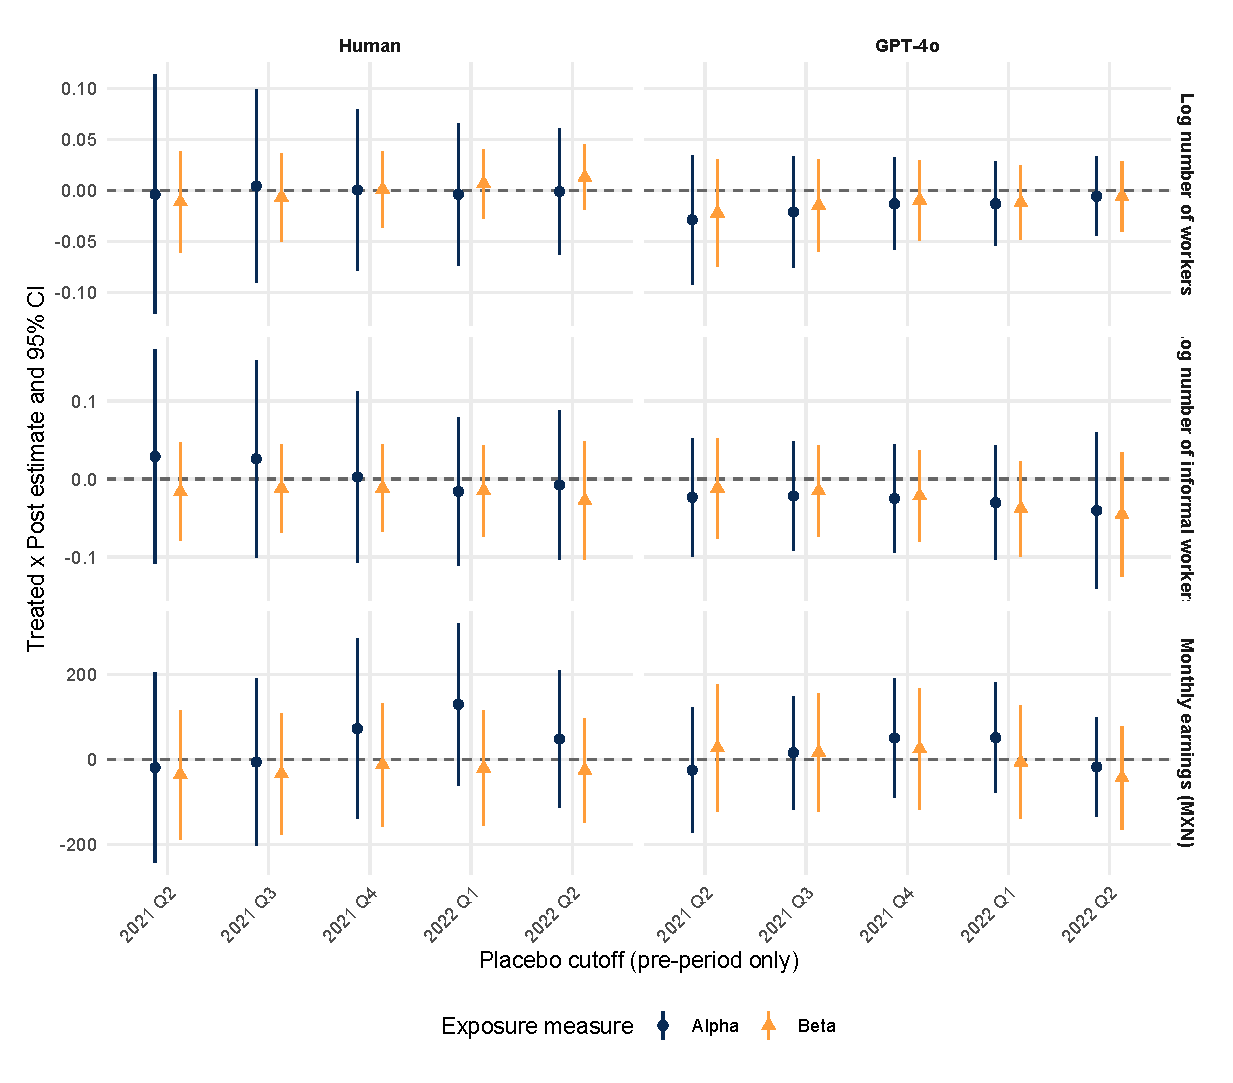
\includegraphics[width=\textwidth]{Figures/placebo_time.eps}

  \begin{minipage}{\textwidth}
    \small
    \textit{Note:} The figure shows placebo tests for every period before treatment in 2022Q4 and measures $\alpha$ and $\beta$. Each estimate plots $\text{Post}_{t} \times \text{ExposureGPT}_j$ for monthly earnings, number of informal workers and number of workers.
  \end{minipage}
\end{figure}